\newpage
\section{HÀM SỐ LƯỢNG GIÁC VÀ ĐỒ THỊ}
\subsection{LÝ THUYẾT CẦN NHỚ}
\subsubsection{Hàm số chẵn, hàm số lẻ}
\begin{boxdn}
Cho hàm số $y = f\left(x\right)$ với tập xác định $\mathrm{D}$
\begin{itemize}
	\item Hàm số $y = f\left(x\right)$ là \textit{hàm số chẵn} nếu $\forall x \in \mathrm{D}$ thì $-x \in \mathrm{D}$ và $f\left(-x\right)=f\left(x\right)$.
	\item Hàm số $y = f\left(x\right)$ là \textit{hàm số lẻ} nếu $\forall x \in \mathrm{D}$ thì $-x \in \mathrm{D}$ và $f\left(-x\right)=-f\left(x\right)$.
\end{itemize}
\end{boxdn}
\begin{luuy}
	Đồ thị hàm số chẵn nhận trục tung làm trục đối xứng, đồ thị hàm số lẻ nhận gốc tọa độ làm tâm đối xứng.
\end{luuy}
\subsubsection{Hàm số tuần hoàn}
\begin{boxdn}
Cho hàm số $y = f\left(x\right)$ với tập xác định $\mathrm{D}$. Hàm số $y = f\left(x\right)$ được gọi là \textit{tuần hoàn} nếu tồn tại một số $T$ khác $0$ sao cho $\forall x \in \mathrm{D}$, ta có
\begin{itemize}
	\item $x+T \in \mathrm{D}$ và $x-T \in \mathrm{D}$;
	\item $f\left(x+T\right) =f\left(x\right)$
\end{itemize}
Số dương $T$ nhỏ nhất (nếu có) thỏa mãn các tính chất trên được gọi là \textit{chu kì} của hàm số tuần hoàn đó.
\end{boxdn}
\subsubsection{Một số hàm số lượng giác cơ bản}

	\begin{enumerate}
		\item Hàm số $y=\sin x$
		\begin{itemize}
			\item Hàm số $y=\sin x$ có tập xác định là $\mathbb{R}$, tập giá trị là đoạn $\left[ -1;1\right]$.
			\item Đồ thị hàm số $y=\sin x$ được biểu diễn ở hình dưới đây
			\begin{center}
				\begin{tikzpicture}[scale=0.8,>=stealth, font=\footnotesize, line join=round, line cap=round]
					\def\xmin{-10} \def\xmax{10.5} \def\ymin{-1.5} \def\ymax{1.8}
					\draw[->] (\xmin,0)--(\xmax,0) node [below]{$x$};
					\draw[->] (0,\ymin)--(0,\ymax) node [right]{$y$};
					\node at (0,0) [below right]{$O$};
					\clip (\xmin+0.1,\ymin+0.1) rectangle (\xmax-0.5,\ymax-0.1);
					\draw[smooth,samples=400,domain=\xmin:\xmax] plot(\x,{sin(\x r)});
					\draw[dashed] (\xmin,1)--(\xmax,1) (\xmin,-1)--(\xmax,-1);
					\foreach \x in {-3*pi,-2.5*pi,-2*pi,-1.5*pi,-pi,-0.5*pi,0}
					{\draw[fill=black] (\x,sin \x*180/pi) circle (1pt);
						\draw[dashed] (\x,sin \x*180/pi)--(\x,0);
						\draw[fill=black] (-\x,sin -\x*180/pi) circle (1pt);
						\draw[dashed] (-\x,sin -\x*180/pi)--(-\x,0);}
					\node at (0,1.3) [left]{$1$};
					\node at (0,-1.3) [left]{$-1$};
					\node at (-2*pi+0.15,0) [below]{$-2\pi$};
					\node at (-3*pi-0.15,0) [below]{$-3\pi$};
					\node at (-2.5*pi,0) [above]{$-\dfrac{5\pi}{2}$};
					\node at (-1.5*pi,0) [below]{$-\dfrac{3\pi}{2}$};
					\node at (-pi-0.15,0) [below]{$-\pi$};
					\node at (-0.5*pi,0) [above]{$-\dfrac{\pi}{2}$};
					\node at (0.5*pi,0) [below]{$\dfrac{\pi}{2}$};
					\node at (pi-0.1,0) [below]{$\pi$};
					\node at (1.5*pi,0) [above]{$\dfrac{3\pi}{2}$};
					\node at (2*pi+0.2,0) [below]{$2\pi$};
					\node at (2.5*pi+0.2,0) [below]{$\dfrac{5\pi}{2}$};
					\node at (3*pi+0.2,0) [below]{$3\pi$};
					\node at (2.5*pi+1,0.8) [above]{$y=\sin x$};
				\end{tikzpicture}
			\end{center}

			\item \textbf{Tính chất:} $y=\sin x$ là hàm số lẻ, có đồ thị đối xứng qua gốc tọa độ $O$; tuần hoàn với chu kì $2\pi$; đồng biến trên mỗi khoảng $\left(-\dfrac{\pi}{2}+k2\pi;\dfrac{\pi}{2}+k2\pi\right)$ và nghịch biến trên mỗi khoảng $\left(\dfrac{\pi}{2}+k2\pi;\dfrac{3\pi}{2}+k2\pi\right) $  với $k \in \mathbb{Z}$
		\end{itemize}
		\item Hàm số $y=\cos x$
		\begin{itemize}
			\item Hàm số $y=\cos x$ có tập xác định là $\mathbb{R}$, tập giá trị là đoạn $\left[ -1;1\right]$.
			\item Đồ thị hàm số $y=\cos x$ được biểu diễn ở hình dưới
			\begin{center}
				\begin{tikzpicture}[scale=0.8,>=stealth, font=\footnotesize, line join=round, line cap=round]
					\def\xmin{-10} \def\xmax{10.5} \def\ymin{-1.5} \def\ymax{1.8}
					\draw[->] (\xmin,0)--(\xmax,0) node [below]{$x$};
					\draw[->] (0,\ymin)--(0,\ymax) node [right]{$y$};
					\node at (0,0) [below right]{$O$};
					\clip (\xmin+0.1,\ymin+0.1) rectangle (\xmax-0.5,\ymax-0.1);
					\draw[smooth,samples=400,domain=\xmin:\xmax] plot(\x,{cos(\x r)});
					\draw[dashed] (\xmin,1)--(\xmax,1) (\xmin,-1)--(\xmax,-1);
					\foreach \x in {-3*pi,-2.5*pi,-2*pi,-1.5*pi,-pi,-0.5*pi,0}
					{\draw[fill=black] (\x,cos \x*180/pi) circle (1pt);
						\draw[dashed] (\x,cos \x*180/pi)--(\x,0);
						\draw[fill=black] (-\x,cos -\x*180/pi) circle (1pt);
						\draw[dashed] (-\x,cos \x*180/pi)--(-\x,0);}
					\node at (0,1.3) [left]{$1$};
					\node at (0,-1.3) [left]{$-1$};
					\node at (-2*pi+0.15,0) [below]{$-2\pi$};
					\node at (-3*pi-0.15,0) [above]{$-3\pi$};
					\node at (-2.5*pi,0) [above]{$-\dfrac{5\pi}{2}$};
					\node at (-1.5*pi,0) [below]{$-\dfrac{3\pi}{2}$};
					\node at (-pi-0.15,0) [above]{$-\pi$};
					\node at (-0.5*pi,0) [above]{$-\dfrac{\pi}{2}$};
					\node at (0.5*pi,0) [below]{$\dfrac{\pi}{2}$};
					\node at (pi-0.1,0) [above]{$\pi$};
					\node at (1.5*pi,0) [above]{$\dfrac{3\pi}{2}$};
					\node at (2*pi+0.2,0) [below]{$2\pi$};
					\node at (2.5*pi+0.2,0) [below]{$\dfrac{5\pi}{2}$};
					\node at (3*pi+0.2,0) [above]{$3\pi$};
					\node at (1.6*pi+1,0.8) [above]{$y=\cos x$};
				\end{tikzpicture}
			\end{center}
			\item \textbf{Tính chất:} $y=\cos x$ là hàm số chẵn, có đồ thị đối xứng qua trục tung; tuần hoàn với chu kì $2\pi$; đồng biến trên mỗi khoảng $\left(-\pi+k2\pi;k2\pi\right)$ và nghịch biến trên mỗi khoảng $\left(k2\pi;\pi+k2\pi\right) $  với $k \in \mathbb{Z}$
		\end{itemize}
		\item Hàm số $y=\tan x$
		\begin{itemize}
			\item Hàm số $y=\tan x$ có tập xác định là $\mathrm{D}=\mathbb{R} \setminus \left\{\dfrac{\pi}{2}+k\pi \,\textbar k\in \mathbb{Z}\right\}$, tập giá trị là $\mathbb{R}$.
			\item Đồ thị hàm số $y=\tan x$ được biểu diễn ở hình dưới
			\begin{center}
				\begin{tikzpicture} [scale=0.8,>=stealth, font=\footnotesize, line join=round, line cap=round]
					\draw[->] (-1.7*pi,0)--(1.6*pi,0) node[below] {$x$};
					\draw[->] (0,-3)--(0,3) node[right]{$y$};
					\draw (0,0) node[below right]{$O$};
					\foreach \i in {-1,0,1}{
						\pgfmathsetmacro{\start}{\i*pi-1.25}
						\pgfmathsetmacro{\left}{(\i-0.5)*pi}
						\pgfmathsetmacro{\end}{\i*pi+1.25}
						\draw[dashed, thin] (\left,-3)--(\left,3);
						\draw[domain=\start:\end, samples=100, smooth] plot (\x, {tan(\x r)});
					}
					\draw[dashed, thin] (1.5*pi,-3)--(1.5*pi,3);
					\node at (-1.5*pi-0.3,0) [below]{$-\dfrac{3\pi}{2}$};
					\node at (-pi-0.3,0) [below right]{$-\pi$};
					\node at (-0.5*pi-0.3,0) [below]{$-\dfrac{\pi}{2}$};
					\node at (0.5*pi-0.1,0) [below]{$\dfrac{\pi}{2}$};
					\node at (pi-0.2,0) [below right]{$\pi$};
					\node at (1.5*pi-0.3,0) [below]{$\dfrac{3\pi}{2}$};
					\node at (pi-0.2,2.5) [above]{$y=\tan x$};
				\end{tikzpicture}
			\end{center}
			\item \textbf{Tính chất:} $y=\tan x$ là hàm số lẻ, có đồ thị đối xứng qua gốc tọa độ $O$; tuần hoàn với chu kì $\pi$; đồng biến trên mỗi khoảng $\left(-\dfrac{\pi}{2}+k\pi;\dfrac{\pi}{2}+k\pi\right)$ với $k \in \mathbb{Z}$
		\end{itemize}
		\item Hàm số $y=\cot x$
		\begin{itemize}
			\item Hàm số $y=\cot x$ có tập xác định là $\mathrm{D}=\mathbb{R} \setminus \left\{k\pi \,\textbar k\in \mathbb{Z}\right\}$, tập giá trị là $\mathbb{R}$.
			\item Đồ thị hàm số $y=\cot x$ được biểu diễn ở hình dưới
			\begin{center}
				\begin{tikzpicture}[scale=0.8,>=stealth, font=\footnotesize, line join=round, line cap=round]
					\def\xmin{-7} \def\xmax{6.5} \def\ymin{-3} \def\ymax{3}
					\draw[->] (\xmin,0)--(\xmax,0) node [below]{$x$};
					\draw[->] (0,\ymin)--(0,\ymax) node [left]{$y$};
					\node at (0,0) [below left]{$O$};
					\clip (\xmin+0.1,\ymin+0.1) rectangle (\xmax-0.5,\ymax-0.1);
					\foreach \n in {-2,-1,0,1}
					{\draw[smooth,samples=400,domain=(\n+0.05)*pi:(\n+0.95)*pi] plot(\x,{1/tan(\x r)});
						\draw[dashed] (\n*pi,\ymin)--(\n*pi,\ymax);}
					\node at (-2*pi-0.4,0) [below]{$-2\pi$};
					\node at (-1.5*pi-0.3,0) [below]{$-\dfrac{3\pi}{2}$};
					\node at (-pi-0.3,0) [below]{$-\pi$};
					\node at (-0.5*pi-0.3,0) [below]{$-\dfrac{\pi}{2}$};
					\node at (0.5*pi-0.1,0) [below]{$\dfrac{\pi}{2}$};
					\node at (pi-0.2,0) [below]{$\pi$};
					\node at (1.5*pi-0.2,0) [below]{$\dfrac{3\pi}{2}$};
					\node at (1.5*pi-0.2,2.5) [above]{$y=\cot x$};
				\end{tikzpicture}
			\end{center}
			\item \textbf{Tính chất:} $y=\cot x$ là hàm số lẻ, có đồ thị đối xứng qua gốc tọa độ $O$;tuần hoàn với chu kì $\pi$; nghịch biến trên mỗi khoảng $\left(k\pi;\pi+k\pi\right)$ với $k \in \mathbb{Z}$
		\end{itemize}
	\end{enumerate}

%-------------------------------------------------------------------------------------------------------------
\subsection{PHÂN LOẠI VÀ PHƯƠNG PHÁP GIẢI TOÁN}
\begin{dang}{Tập xác định của hàm số lượng giác}
	\textbf{Phương pháp giải}
	Ta chú ý một số điều kiện sau:
	\begin{enumerate}
		\item $y=\dfrac{f(x)}{g(x)}$ xác định $ \Leftrightarrow g(x)\ne 0$.
		\item $y=\sqrt[2n]{f(x)}$ xác định $ \Leftrightarrow f(x)\geqslant 0$, trong đó $n\in \mathbb{N}^*$.
		\item $y=\dfrac{g(x)}{\sqrt[2n]{f(x)}}$ xác định $\Leftrightarrow f(x) >0$ trong đó $n\in \mathbb{N}^* $
		\item $y=\tan \left[u(x)\right]$ xác định $ \Leftrightarrow u(x)$ xác định và $u(x)\ne \dfrac{\pi}{2}+k\pi,k\in \mathbb{Z}$.
		\item $y=\cot \left[u(x)\right]$ xác định $ \Leftrightarrow u(x)$ xác định và $u(x)\ne k\pi,k\in \mathbb{Z}$.
	\end{enumerate}
\end{dang}
\begin{vd}%[1D1H4-2]%[Dự án đề cương 2025]%[Đoàn Minh Tâm]
	Tìm tập xác định của hàm số
	\begin{enumEX}{3}
		\item $y=1-\cos 4x$.
		\item $y=\dfrac{2+\sin\left(\dfrac{\pi}{3}-x\right)}{x}$.
		\item $y=\cot x$.
		\item  $y=\tan 2x$.
		\item $y=\tan\left(x+\dfrac{\pi}{4}\right)$.
		\item $y=\cot \left(60^\circ - 3x\right)$.
	\end{enumEX}
	\loigiai{
		\begin{enumerate}
			\item Tập xác định $\mathscr{D}=\mathbb{R} $.
			\item Tập xác định $\mathscr{D}=\mathbb{R} \setminus \{0\} $.
			\item Tập xác định $\mathscr{D}=\mathbb{R} \setminus \left\{ k\pi|k\in \mathbb{Z} \right\} $.
			\item Điều kiện xác định: $2x\neq \dfrac{\pi}{2}+k\pi\Leftrightarrow x\neq \dfrac{\pi}{4}+k\dfrac{\pi}{2}$, $k\in \mathbb{Z}$.\\
			Tập xác định $\mathscr{D}=\mathbb{R} \setminus \left\{ \dfrac{\pi}{4}+k\dfrac{\pi}{2}|k\in \mathbb{Z} \right\}$.
			\item Điều kiện xác định của hàm số $y=\tan\left(x+\dfrac{\pi}{4}\right)$ là
			\[\cos \left(x+\dfrac{\pi}{4}\right)\neq0\Leftrightarrow x+\dfrac{\pi}{4}\ne \dfrac{\pi}{2}+k\pi\Leftrightarrow x\ne \dfrac{\pi}{4}+k\pi\,(k\in\mathbb{Z}).\]
			Vậy tập xác định của hàm số $y=\tan\left(x+\dfrac{\pi}{4}\right)$ là $\mathscr{D}=\mathbb{R}\backslash\left\{\dfrac{\pi}{4}+k\pi\,|(k\in\mathbb{Z})\right\}$.
			\item Điều kiện xác định của hàm số $y=\cot\left(60^\circ - 3x\right)$ là
			\[60^\circ - 3x \ne k 180^\circ\Leftrightarrow x\ne 20^\circ -k \cdot 60^\circ,(k\in\mathbb{Z}).\]
			Vậy tập xác định của hàm số $y=\cot\left(60^\circ - 3x\right)$ là $\mathscr{D}=\mathbb{R}\backslash\left\{20^\circ -k \cdot 60^\circ\,|(k\in\mathbb{Z})\right\}$.
		\end{enumerate}
	}
\end{vd}
\begin{dang}{Tìm tập giá trị và min - max}
		\textbf{Phương pháp giải}
	\begin{itemize}
		\item Dựa vào tập giá trị của hàm số lượng giác, chẳng hạn
		\begin{itemize}
			\item $ - 1\leq\sin x\leq 1\Rightarrow \hoac{& 0 \leq|\sin x| \leq 1\\ & 0\leq\sin^2x\leq 1}$ hoặc $ - 1\leq\cos x\leq 1\Rightarrow \hoac{& 0\leq|\cos x|\leq 1\\ & 0\leq\cos^2x\leq 1.}$
			\item Biến đổi đưa về dạng $m\leq y\leq M$.
		\end{itemize}
		\item  Kết luận $\max y=M$ và $\min y=m$.
	\end{itemize}
\end{dang}
\begin{vd}%[1D1H4-6]%[Dự án đề cương 2025]%[Đoàn Minh Tâm]
	Tìm giá trị lớn nhất và giá trị nhỏ nhất của các hàm số sau
	\begin{enumEX}{2}
		\item $y=2\cos x+3$.
		\item $y=3\sin^22x-4$.
	\end{enumEX}
	\loigiai{
		\begin{enumerate}
			\item Do $-1\leq\cos x\leq 1$ nên $ 1\leq 2\cos x+3\leq 5$.
			\begin{itemize}
				\item $y=1$ khi $\cos x =-1$, luôn tồn tại $x$ thỏa mãn, chẳng hạn $x=-\pi$.
				\item $y=5$ khi $\cos x =1$, luôn tồn tại $x$ thỏa mãn, chẳng hạn $x=0$.
			\end{itemize}
			Vậy $\min y=1$ và $\max y=5$.
			\item Do $0\leq\sin^22x\leq 1$ nên $ - 4\leq y=3\sin^22x - 4\leq - 1$.
			\begin{itemize}
				\item  $y=-4$ khi $\sin 2x =0$, luôn tồn tại $x$ thỏa mãn, chẳng hạn $x=0$.
				\item $y=-1$ khi $\sin^22x =1$, luôn tồn tại $x$ thỏa mãn, chẳng hạn $x=\dfrac{\pi}{4}$.
			\end{itemize}
			Vậy $\min y=-4$ và $\max y=-1$.
		\end{enumerate}
	}
\end{vd}
\begin{vd}%[1D1V4-6]%[1T1K4-5]%[Dự án đề cương 2025]%[Đoàn Minh Tâm]
	Tìm giá trị lớn nhất và giá trị nhỏ nhất của các hàm số: $y= - \sin^2x - \cos x + 2$.
	\loigiai{
		Ta có: $y= - \sin^2x - \cos x + 2= - \left(1 - \cos^2x\right) - \cos x + 2=\cos^2x - \cos x + 1$\\
		{\bf{Cách 1:}} $y=\left(\cos x - \dfrac{1}{2}\right)^2 + \dfrac{3}{4}.$\\
		Do $ - 1\leq\cos x\leq 1$ nên $ - \dfrac{3}{2}\leq\cos x - \dfrac{1}{2}\leq\dfrac{1}{2}$.\\
		Suy ra $0\leq\left(\cos x - \dfrac{1}{2}\right)^2\leq\dfrac{9}{4}\Leftrightarrow \dfrac{3}{4}\leq y\leq 3$.\\
		$\circ$ $y=\dfrac{3}{4}$ khi $\cos x =\dfrac{1}{2}$, luôn tồn tại $x$ thỏa mãn, chẳng hạn $x=\dfrac{\pi}{3}$.\\
		$\circ$ $y=3$ khi $\cos x =-1$, luôn tồn tại $x$ thỏa mãn, chẳng hạn $x=\pi$.\\
		Vậy $\min y=\dfrac{3}{4}$ và $\max y=3$.\\
		{\bf{Cách 2:}} Đặt $t=\cos x$, $-1\le t\le 1$. Khi đó: $y=t^2-t+1$, $-1\le t\le 1$.\\
		Bảng biến thiên
		\begin{center}
			
\begin{tikzpicture}[>=stealth]
				\tkzTabInit[lgt=1.5,espcl=3]
				{$t$/1,$y$/1.7}
				{$-1$,$\dfrac{1}{2}$,$1$}
				\tkzTabVar{+/$3$,-/$\dfrac{3}{4}$,+/$1$}
			\end{tikzpicture}
		\end{center}
		Vậy $\min y=\dfrac{3}{4}$ và $\max y=3$.
	}
\end{vd}
\begin{dang}{Dựa vào đồ thị để tính giá trị của hàm số, xét sự tương giao}
	\textbf{Phương pháp giải}
	Dựa vào đồ thị của hàm số và đồ thị của các hàm số tương ứng vẽ trên cùng một hệ trục tọa độ và xét sự tương giao dẫn đến tìm ra giá trị $ x $ thỏa mãn yêu cầu đề bài.
\end{dang}
	\begin{vd}%[1D1H4-7]%[Dự án đề cương 2025]%[Đoàn Minh Tâm]
	Dùng đồ thị hàm số, tìm giá trị của $x$ trên đoạn $[-2 \pi ; 2 \pi]$ để
	\begin{enumerate}
		\item 	Hàm số $y=\sin x$ nhận giá trị bằng $1$.
		\item 	Hàm số $y=\sin x$ nhận giá trị bằng $0$.
		\item 	Hàm số $y=\cos x$ nhận giá trị bằng $-1$.
		\item 	Hàm số $y=\cos x$ nhận giá trị bằng $0$.
	\end{enumerate}

	\loigiai{
		Trên đoạn $[-2 \pi ; 2 \pi]$
		\begin{enumerate}
			\item Hàm số $y=\sin x$ nhận giá trị bằng $1$ với $x \in\left\{-\dfrac{3 \pi}{2} ; \dfrac{\pi}{2}\right\}$.
			\item Hàm số $y=\sin x$ nhận giá trị bằng $0$ với $x \in\{-2 \pi ;-\pi ; 0 ; \pi ; 2 \pi\}$.
			\item Hàm số $y=\cos x$ nhận giá trị bằng $-1$ với $x \in\{-\pi ; \pi\}$.
			\item Hàm số $y=\cos x$ nhận giá trị bằng 0 với $x \in\left\{-\dfrac{3 \pi}{2} ;-\dfrac{\pi}{2} ; \dfrac{\pi}{2} ; \dfrac{3 \pi}{2}\right\}$.
		\end{enumerate}
	}
\end{vd}
\begin{vd}%[1D1V4-7]%[Dự án đề cương 2025]%[Đoàn Minh Tâm]
	Dùng đồ thị hàm số, hãy cho biết:
	\begin{enumerate}
		\item 	Với mỗi $m \in[-1 ; 1]$, có bao nhiêu giá trị $\alpha \in\left[-\dfrac{\pi}{2} ; \dfrac{\pi}{2}\right]$ sao cho $\sin \alpha=m$.
		\item 	Với mỗi $m \in \mathbb{R}$, có bao nhiêu giá trị $\alpha \in\left(-\dfrac{\pi}{2} ; \dfrac{\pi}{2}\right)$ sao cho tan $\alpha=m$.
	\end{enumerate}
	\loigiai{
		\begin{enumerate}
			\item Số giá trị $\alpha \in\left[-\dfrac{\pi}{2} ; \dfrac{\pi}{2}\right]$ sao cho $\sin \alpha=m$ bằng số giao điểm của đồ thị hàm số $y=\sin x$ trên đoạn $\left[-\dfrac{\pi}{2} ; \dfrac{\pi}{2}\right]$ và đường thẳng $y=m$.\\
			Căn cứ vào đồ thị hàm số, với mỗi $m \in[-1 ; 1]$, có đúng một giá trị $\alpha \in\left[-\dfrac{\pi}{2} ; \dfrac{\pi}{2}\right]$ sao cho $\sin \alpha=m$.
			\item Số giá trị $\alpha \in\left(-\dfrac{\pi}{2} ; \dfrac{\pi}{2}\right)$ sao cho $\tan \alpha=m$ bằng số giao điểm của đồ thị hàm số $y=\tan x$ trên khoảng $\left(-\dfrac{\pi}{2} ; \dfrac{\pi}{2}\right)$ và đường thẳng $y=m$.\\
			Căn cứ vào đồ thị hàm số, với mỗi $m \in \mathbb{R}$, có đúng một giá trị $\alpha \in\left(-\dfrac{\pi}{2} ; \dfrac{\pi}{2}\right)$ sao cho $\tan \alpha=m$.
		\end{enumerate}
	}
\end{vd}
\begin{dang}{Xét sự đồng biến, nghịch biến của hàm số lượng giác}
	\textbf{Phương pháp giải}
	Ta chú ý các tính chất sau
	\begin{enumerate}
		\item Hàm số $y=\sin x$ đồng biến trên mỗi khoảng $\left(-\dfrac{\pi}{2}+k2\pi;\dfrac{\pi}{2}+k2\pi\right)$ $(k \in \mathbb{Z})$ và nghịch biến trên mỗi khoảng $\left(\dfrac{\pi}{2}+k2\pi;\dfrac{3\pi}{2}+k2\pi\right)$ $(k \in \mathbb{Z})$.
		\item Hàm số $y=\cos x$ đồng biến trên mỗi khoảng $\left(-\pi+k2\pi; k2\pi\right)$ $(k \in \mathbb{Z})$ và nghịch biến trên mỗi khoảng $\left(k2\pi;\pi+k2\pi\right)$ $(k \in \mathbb{Z})$.
		\item Hàm số $y=\tan x$ đồng biến trên mỗi khoảng $\left(-\dfrac{\pi}{2}+k\pi;\dfrac{\pi}{2}+k\pi\right)$ $(k \in \mathbb{Z})$.
		\item Hàm số $y=\cot x$ nghịch biến trên mỗi khoảng $\left(k\pi;\pi+k\pi\right)$ $(k \in \mathbb{Z})$.
	\end{enumerate}
\end{dang}
\begin{vd}%[1D1H4-3] %[Dự án đề cương 2025]%[Đoàn Minh Tâm]
	Xét sự biến thiên của mỗi hàm số sau trên các khoảng tương ứng:
	\begin{enumerate}
		\item 	$y=\sin x$ trên khoảng $\left(-\dfrac{9 \pi}{2} ;-\dfrac{7 \pi}{2}\right),\left(\dfrac{21 \pi}{2} ; \dfrac{23 \pi}{2}\right)$;
		\item 	$y=\cos x$ trên khoảng $(-20 \pi ;-19 \pi),(-9 \pi ;-8 \pi)$.
	\end{enumerate}
	\loigiai{
		\begin{enumerate}
			\item Ta có
			\begin{itemize}
				\item $\left( -\dfrac{9\pi }{2};-\dfrac{7\pi }{2} \right)=\,\left( -\dfrac{\pi }{2}-4\pi ;\dfrac{\pi }{2}-4\pi  \right)$.\\
				Do hàm số $y=\sin x$ đồng biến trên khoảng $\left(-\dfrac{\pi}{2};\dfrac{\pi}{2}\right)$ nên hàm số đó cũng đồng biến trên khoảng $\left(-\dfrac{9\pi}{2};-\dfrac{7\pi}{2}\right)$.
				\item $\left( \dfrac{21\pi }{2};\dfrac{23\pi }{2} \right)=\left( \dfrac{\pi }{2}+10\pi ;\dfrac{3\pi }{2}+10\pi  \right)$.\\
				Do hàm số $y=\sin x$ nghịch biến trên khoảng $\left(\dfrac{\pi}{2};\dfrac{3\pi}{2}\right)$ nên hàm số đó cũng nghịch biến trên khoảng $\left(\dfrac{21\pi}{2};\dfrac{23\pi}{2}\right)$ .
			\end{itemize}
			\item Ta có
			\begin{itemize}
				\item $\left( -20\pi ;-19\pi  \right)=\left( 0-20\pi ;\pi -20\pi  \right)$.\\
				Do hàm số $y=\cos x$ nghịch biến trên khoảng $\left(0;\pi\right)$ nên hàm số đó cũng nghịch biến trên khoảng $\left(-20\pi ;-19\pi\right)$
				\item $\left( -9\pi ;-8\pi  \right)=\left( -\pi -8\pi ;0-8\pi  \right)$.\\
				Do hàm số $y=\cos x$ đồng biến trên khoảng $\left(-\pi ;0\right)$ nên hàm số đó cũng đồng biến trên khoảng $\left(-9\pi ;-8\pi\right)$
			\end{itemize}
		\end{enumerate}
	}
\end{vd}
\begin{dang}{Xét tính chẵn, lẻ của hàm số}
		\textbf{Phương pháp giải}
	\begin{itemize}
		\item \textbf{Bước 1.} Tìm tập xác định $\mathscr{D}$ của hàm số lượng giác.\\
		Nếu $\forall x\in \mathscr{D}$ thì $ - x\in \mathscr{D}$, chuyển sang bước 2.
		\item  \textbf{Bước 2.} Tính $f(-x)$, nghĩa là sẽ thay $x$ bằng $-x$, sẽ có 2 kết quả thường gặp sau
		\begin{itemize}
			\item Nếu $f( - x)=f(x)\Rightarrow f(x)$ là hàm số chẵn.
			\item Nếu $f( - x)= - f(x)\Rightarrow f(x)$ là hàm số lẻ.
		\end{itemize}
	\end{itemize}
	\begin{luuy}
		\begin{itemize}
			\item Nếu tồn tại $x\in \mathscr{D}$ và $-x\notin \mathscr{D}$ hoặc $f( - x)$ không bằng $f(x)$ hay $ - f(x)$ ta sẽ kết luận hàm số không chẵn, không lẻ.
			\item Ta thường sử dụng cung góc liên kết dạng cung đối trong dạng toán này, cụ thể:\\
			$\cos( - a)=\cos a$, $\sin( - a)= - \sin a$, $\tan( - a)= - \tan a$, $\cot( - a)= - \cot a$.
			\item Hàm số $y=\cos x$ là hàm số chẵn, hàm số $y=\sin x$, $y=\tan x$, $y=\cot x$ là các hàm số lẻ.
		\end{itemize}
	\end{luuy}
\end{dang}
\begin{vd}%[1D1H4-4] %[Dự án đề cương 2025]%[Đoàn Minh Tâm]
	Xét tính chẵn, lẻ của các hàm số
	\begin{enumEX}{3}
		\item $y=\sin x\cdot\cos x$;
		\item $y=\tan x+\cot x$;
		\item $y=\sin^2x$.
	\end{enumEX}
	\loigiai{
		\begin{enumerate}
			\item Hàm số $y=f(x)=\sin x\cdot\cos x$ là hàm số lẻ vì
			\begin{itemize}
				\item Tập xác định là $D=\mathbb{R}$.
				\item $\forall x\in \mathbb{R}$ thì $-x\in\mathbb{R}$ và $f\left(-x\right)=\sin\left(-x\right)\cdot\cos\left(-x\right)=-\left(\sin x\cdot\cos x\right)=-f(x)$.
			\end{itemize}
			\item Hàm số $y=g(x)=\tan x+\cot x$ là hàm số lẻ vì:
			\begin{itemize}
				\item Tập xác định là $D=\mathbb{R}\setminus\left\{\dfrac{\pi}{2}\big|k\in\mathbb{Z}\right\}$.
				\item $\forall x\in \mathbb{R}$ thì $-x\in D$ và $g\left(-x\right)=\tan\left(-x\right)+\cot\left(-x\right)=-\left(\tan x+\cot x\right)=-g(x)$.
			\end{itemize}
			\item Hàm số $y=h(x)=\sin^2x$ là hàm số chẵn vì:
			\begin{itemize}
				\item Tập xác định là $D=\mathbb{R}$.
				\item $\forall x\in \mathbb{R}$ thì $-x\in\mathbb{R}$ và $h\left(-x\right)=\sin^2\left(-x\right)=\left(-\sin x\right)^2=\sin^2x=h(x)$.
			\end{itemize}
		\end{enumerate}
	}
\end{vd}

\begin{dang}{Ứng dụng hàm số lượng giác và đồ thị trong bài toán thực tiễn}
	 Mô hình hóa bài toán thực tiễn và dùng các phương pháp của các dạng toán về hàm số lượng giác và đồ thị để giải bài toán.
\end{dang}
\begin{vd}%[1D1H4-8] %[Dự án đề cương 2025]%[Đoàn Minh Tâm]
	Một dao động điều hoà có phương trình li độ dao động là: $x=A\cos\left(\omega\,t+\varphi\right)$ , trong đó $t$ là thời gian tính bằng giây, $A$ là biên độ dao động và $x$ là li độ dao động đều được tính bằng centimét, $\omega >0$ . Khi đó, chu kì $T$ của dao động là $T=\dfrac{2\pi}{\omega}$ . Xác định giá trị của li độ khi $t=0$, $t=\dfrac{T}{4}$, $t=\dfrac{T}{2}$, $t=\dfrac{3T}{4}$, $t=T$ và vẽ đồ thị biểu diễn li độ của dao động điều hoà trên đoạn $\left[0;2T\right]$ trong các trường hợp:
	\begin{enumerate}
		\item $A=3$ cm, $\varphi=0$;
		\item $A=3$ cm, $\varphi=-\dfrac{\pi}{2}$;
		\item $A=3$ cm, $\varphi=\dfrac{\pi}{2}$.
	\end{enumerate}
	\loigiai{
		%		\begin{figure}
		\begin{enumerate}
			\item Khi $A=3cm,\,\,\varphi=0$, ta có: $x=3\cos\left(\omega\,t\right)=3\cos\left(\dfrac{2\pi}{T}t\right)$.\\
			\immini
			{Ta có bảng xác định giá trị li độ tại một số thời điểm và đồ thị cần vẽ ở Hình 9:\\
				\begin{tabular}{|c|c|c|c|c|c|}
					\hline
					$t$ &$0$  &$\dfrac{T}{4}$  &$\dfrac{T}{2}$  &$\dfrac{3T}{4}$  &$T$  \\
					\hline
					$x$ &$3$  &$0$  &$-3$  &$0$  &$3$  \\
					\hline
				\end{tabular}
			}{
				\begin{tikzpicture} [scale=0.6,>=stealth, font=\footnotesize, line join=round, line cap=round]
					\draw[->] (0,0)--(4*pi+0.5,0) node[above] {$t$};
					\draw[->] (0,-3.5)--(0,3.5) node[below left]{$x$};
					\draw (0,0) node[below left]{$O$};
					\def\xmin{0} \def\xmax{4*pi}
					\draw[domain=\xmin:\xmax,samples=100, smooth] plot (\x, {3*cos(\x r)});
					\draw[dashed] (\xmin,3)--(\xmax+0.5,3) (\xmin,-3)--(\xmax+0.5,-3);
					\node at (0.5*pi,0) [below left]{$\dfrac{T}{4}$};
					\node at (pi,0) [above]{$\dfrac{T}{2}$};
					\node at (1.5*pi,0) [below right]{$\dfrac{3T}{4}$};
					\node at (2*pi,0) [below]{$T$};
					\node at (2.5*pi,0) [below left]{$\dfrac{5T}{4}$};
					\node at (3*pi,0) [above]{$\dfrac{3T}{2}$};
					\node at (3.5*pi,0) [below right]{$\dfrac{7T}{4}$};
					\node at (4*pi,0) [below]{$2T$};
					\draw[dashed] (pi,0)--(pi,-3);
					\draw[dashed] (2*pi,0)--(2*pi,3);
					\draw[dashed] (3*pi,0)--(3*pi,-3);
					\draw[dashed] (4*pi,0)--(4*pi,3);
				\end{tikzpicture}
				%			\caption{}
			}
			\item Khi $A=3cm,\,\,\varphi=-\dfrac{\pi}{2}$, ta có: $x=3\cos\left(\omega\,t-\dfrac{\pi}{2}\right)=3\cos\left(\dfrac{2\pi}{T}t-\dfrac{\pi}{2}\right)$.
			\immini
			{Ta có bảng xác định giá trị li độ tại một số thời điểm và đồ thị cần vẽ ở Hình 10:\\
				\begin{tabular}{|c|c|c|c|c|c|}
					\hline
					$t$ &$0$  &$\dfrac{T}{4}$  &$\dfrac{T}{2}$  &$\dfrac{3T}{4}$  &$T$  \\
					\hline
					$x$ &$0$  &$3$  &$0$  &$-3$    &$0$  \\
					\hline
				\end{tabular}
			}
			{
				\begin{tikzpicture} [scale=0.6,>=stealth, font=\footnotesize, line join=round, line cap=round]
					\draw[->] (0,0)--(4*pi+0.5,0) node[above] {$t$};
					\draw[->] (0,-3.5)--(0,3.5) node[below left]{$x$};
					\draw (0,0) node[below left]{$O$};
					\def\xmin{0} \def\xmax{4*pi}
					\draw[domain=\xmin:\xmax,samples=100, smooth] plot (\x, {3*cos((\x-0.5*pi) r)});
					\draw[dashed] (\xmin,3)--(\xmax+0.5,3) (\xmin,-3)--(\xmax+0.5,-3);
					\node at (0.5*pi,0) [below left]{$\dfrac{T}{4}$};
					\node at (pi,0) [below left]{$\dfrac{T}{2}$};
					\node at (1.5*pi,0) [above]{$\dfrac{3T}{4}$};
					\node at (2*pi,0) [below right]{$T$};
					\node at (2.5*pi,0) [below]{$\dfrac{5T}{4}$};
					\node at (3*pi,0) [below left]{$\dfrac{3T}{2}$};
					\node at (3.5*pi,0) [above]{$\dfrac{7T}{4}$};
					\node at (4*pi,0) [below right]{$2T$};
					\draw[dashed] (0.5*pi,0)--(0.5*pi,3);
					\draw[dashed] (1.5*pi,0)--(1.5*pi,-3);
					\draw[dashed] (2.5*pi,0)--(2.5*pi,3);
					\draw[dashed] (3.5*pi,0)--(3.5*pi,-3);
				\end{tikzpicture}
				%			\caption{}
			}
			\item Khi $A=3cm,\,\,\varphi=\dfrac{\pi}{2}$, ta có: $x=3\cos\left(\omega\,t+\dfrac{\pi}{2}\right)=3\cos\left(\dfrac{2\pi}{T}t+\dfrac{\pi}{2}\right)$.
			\immini
			{Ta có bảng xác định giá trị li độ tại một số thời điểm và đồ thị cần vẽ ở Hình 11:\\
				\begin{tabular}{|c|c|c|c|c|c|}
					\hline
					$t$ &$0$  &$\dfrac{T}{4}$  &$\dfrac{T}{2}$  &$\dfrac{3T}{4}$  &$T$  \\
					\hline
					$x$ &$0$  &$-3$  &$0$  &$3$    &$0$  \\
					\hline
				\end{tabular}
			}
			{
				\begin{tikzpicture} [scale=0.6,>=stealth, font=\footnotesize, line join=round, line cap=round]
					\draw[->] (0,0)--(4*pi+0.5,0) node[above] {$t$};
					\draw[->] (0,-3.5)--(0,3.5) node[below left]{$x$};
					\draw (0,0) node[below left]{$O$};
					\def\xmin{0} \def\xmax{4*pi}
					\draw[domain=\xmin:\xmax,samples=100, smooth] plot (\x, {3*cos((\x+0.5*pi) r)});
					\draw[dashed] (\xmin,3)--(\xmax+0.5,3) (\xmin,-3)--(\xmax+0.5,-3);
					\node at (0.5*pi,0) [above]{$\dfrac{T}{4}$};
					\node at (pi,0) [below right]{$\dfrac{T}{2}$};
					\node at (1.5*pi,0) [below]{$\dfrac{3T}{4}$};
					\node at (2*pi,0) [below left]{$T$};
					\node at (2.5*pi,0) [above]{$\dfrac{5T}{4}$};
					\node at (3*pi,0) [below right]{$\dfrac{3T}{2}$};
					\node at (3.5*pi,0) [below]{$\dfrac{7T}{4}$};
					\node at (4*pi,0) [below]{$2T$};
					\draw[dashed] (0.5*pi,0)--(0.5*pi,-3);
					\draw[dashed] (1.5*pi,0)--(1.5*pi,3);
					\draw[dashed] (2.5*pi,0)--(2.5*pi,-3);
					\draw[dashed] (3.5*pi,0)--(3.5*pi,3);
				\end{tikzpicture}
				%			\caption{}
			}
		\end{enumerate}
		%	\end{figure}
	}
\end{vd}

\begin{vd}%[1D1V4-8] %[Dự án đề cương 2025]%[Đoàn Minh Tâm]
		Một vòng quay trò chơi có bán kính $57m$, trục quay cách mặt đất $57{,}5m$, quay đều mỗi vòng hết $15$ phút. Khi vòng quay quay đều, khoảng cách $ h$ ( m ) từ một cabin gắn tại điểm $A$ của vòng quay đến mặt đất được tính bởi công thức: $ h( t )=57\sin \left( \dfrac{2\pi }{15}t-\dfrac{\pi }{2} \right)+57{,}5$ với $ t$ là thời gian quay của vòng quay tính bằng phút $( t\ge 0 )$ (Hình 12)
		\begin{center}
			\begin{tikzpicture}[scale=0.8, line join=round, line cap=round]
				\def\r{sqrt(5)}
				\coordinate[label=above:$O$] (O) at (0,0);
				\draw[name path=(C)] (O) circle (\r);
				\coordinate (M) at (0,-2.5);
				\draw ($(M)!3cm!90:(O)$)--($(M)!3cm!-90:(O)$);
				\draw[smooth] (O)--(M);
				\coordinate[label=right:$A$] (A) at (2,1);
				\draw[smooth] (O)--(A);
				\draw[dashed,smooth] (2,-2.5)--(2,1);
				\draw (2,-0.5) node[left] {$h$};
				\draw (0,-1) node[left] {$57,5 m$};
				\draw (1.25,0.75) node[left] {$57 m$};
			\end{tikzpicture}
		\end{center}
	\begin{enumerate}
		\item Tính chu kỳ của hàm số $ h( t )$?
		\item Khi $ t=0$ (phút) thì khoảng cách từ ca bin đến mặt đất là bao nhiêu?
		\item Khi quay một vòng lần thứ nhất tính từ thời điểm $ t=0$ (phút), tại thời điểm nào của $ t$ thì cabin ở vị trí cao nhất? Ở Vị trí đạt được chiều cao là $86m?$.
	\end{enumerate}
	\loigiai{
		\begin{enumerate}
			\item Vì vòng quay trò chơi quay mỗi vòng hết $15$ phút nên chu kì của hàm số $ h( t )$ bằng $15$ phút.
			\item Khi $ t=0$ thì $ h=57\sin \left( -\dfrac{\pi }{2} \right)+57{,}5=0{,}5( m )$. Vậy khi đó khoảng cách từ cabin đến mặt đất bằng $0{,}5m$.
			\item Khi quay một vòng, cabin ở vị trí cao nhất khi $\sin \left( \dfrac{2\pi }{15}t-\dfrac{\pi }{2} \right)=1$ hay $ t=7{,}5$ (phút); cabin đạt được chiều cao là $86m$ lần đầu tiên $ t=5$ (phút).
		\end{enumerate}
	}
\end{vd}

%-----------------------------------------------------------------------------
\subsection{Bài tập rèn luyện}
\ind{PHẦN I.} \inden{Câu trắc nghiệm nhiều phương án lựa chọn. Mỗi câu hỏi học sinh chỉ chọn một phương án.}\\
\setcounter{ex}{0}
\Opensolutionfile{ans}[ans/1D1-Bai3-TN]%--Đặt tên 2D1-Bai1-Dang1-TN
\begin{ex}[Trích đề thi GHKI - Trường Nguyễn Bỉnh Khiêm - Hà Nội - Năm học 2024-2025]%[1D1N4-4]%[Dự án đề cương 2025]%[Đoàn Minh Tâm]%Câu 1
	Trong các mệnh đề sau, mệnh đề nào đúng?
	\choice
	{Hàm số $y=\cot x$ là hàm số chẵn}
	{\True Hàm số $y=\cos x$ là hàm số chẵn}
	{Hàm số $y=\sin x$ là hàm số chẵn}
	{Hàm số $y=\tan x$ là hàm số chẵn}
	\loigiai{
		Hàm số $y=\cos x$ là hàm số chẵn là mệnh đề đúng.
	}
\end{ex}

\begin{ex}[Trích đề thi GHKI - Trường Nguyễn Trân - Bình Định - Năm học 2023-2024]%[1D1N4-4]%[Dự án đề cương 2025]%[Đoàn Minh Tâm]%Câu 1
	Cho các hàm số $y=\cos x$, $y=\sin x$, $y=\tan x$, $y=\cot x$. Trong các hàm số trên, có bao nhiêu hàm số lẻ?
	\choice
	{$1$}
	{\True $3$}
	{$2$}
	{$4$}
	\loigiai{
		Các hàm số  $y=\sin x$, $y=\tan x$, $y=\cot x$ là các hàm số lẻ.
	}
\end{ex}

\begin{ex}[Trích đề thi GHKI - Trường Chuyên Bình Thuận - Năm học 2024-2025]%[1D1N4-2]%[Dự án đề cương 2025]%[Đoàn Minh Tâm]%Câu 2
	Hàm số nào sau đây có tập xác định là tập số thực $\mathbb{R}$?
	\choice
	{ $y=\dfrac{\sin x}{2 \cos x-1}$}
	{ $y=\dfrac{2 \cot x}{\cos x-2}$}
	{ $y=\dfrac{2 \cos x}{3 \sin x-2}$}
	{\True $y=\dfrac{2}{2 \sin x-3}$}
	\loigiai{
		Hàm số $y=\dfrac{2}{2 \sin x-3}$ có tập xác định là tập số thực $\mathbb{R}$.
	}
\end{ex}

\begin{ex}[Trích đề thi GHKI - Trường Trần Phú - Năm học 2023-2024]%[1D1N4-3]%[Dự án đề cương 2025]%[Đoàn Minh Tâm]%Câu 3
	Cho hàm số $y = \sin 2023x$. Khẳng định nào sau đây là đúng?
	\choice
	{Giá trị nhỏ nhất của hàm số bằng $0$}
	{Giá trị nhỏ nhất của hàm số bằng $-2023$}
	{Giá trị lớn nhất của hàm số bằng $2023$}
	{\True Giá trị lớn nhất của hàm số bằng $1$}
	\loigiai{
		Ta có $-1 \leq \sin(2023x) \leq 1$. \\
		Nên giá trị lớn nhất của $y= \sin (2023x)$ bằng $1$.
	}
\end{ex}

\begin{ex}[Trích đề thi GHKI - Trường Nguyễn An Ninh - Năm học 2024-2025]%[1D1N4-1]%[Dự án đề cương 2025]%[Đoàn Minh Tâm]%Câu 3
	Khẳng định nào sau đây là \textbf{sai}?
	\choice
	{$\sin(x + k2\pi) = \sin x$, $\forall k \in \mathbb{Z}$, $\forall x \in \mathbb{R}$}
	{\True Hàm số $y = \sin x$ là hàm số chẵn trên tập xác định}
	{$-1 \leq \sin x \leq 1$, $\forall x \in \mathbb{R}$}
	{Tập xác định của hàm số $y = \sin x$ là $\mathbb{R}$}
	\loigiai{
		Hàm số $y = \sin x$ là hàm số lẻ trên tập xác định $\mathbb{R}$.
	}
\end{ex}

\begin{ex}[Trích đề thi GHKI - Trường Nguyễn Thị Minh Khai - Năm học 2024-2025]%[1D1N4-5]%[Dự án đề cương 2025]%[Đoàn Minh Tâm]%Câu 4
	Hàm số $y=\tan x$ tuần hoàn với chu kì $T$ nào sau đây?
	\choice
	{$T=4\pi$}
	{$T=3\pi$}
	{$T=2\pi$}
	{\True $T=\pi$}
	\loigiai{
		Hàm số $y=\tan\left(ax+b\right)$ tuần hoàn với chu kì $T=\dfrac{\pi}{|a|}$.\\
		Vậy hàm số $y=\tan x$ tuần hoàn với chu kì $T=\pi$.
	}
\end{ex}

\begin{ex}[Trích đề thi GHKI - Trường Thường Tín - Hà Nội - Năm học 2023-2024]%[1D1N4-3]%[Dự án đề cương 2025]%[Đoàn Minh Tâm]%Câu 4
	Hàm số $y=\sin x$ đồng biến trên khoảng nào?
	\choice
	{$\left(\dfrac{\pi}{2}; \dfrac{3\pi}{2}\right)$}
	{$(0; \pi)$}
	{$(-\pi; 0)$}
	{\True $\left(-\dfrac{\pi}{2}; \dfrac{\pi}{2}\right)$}
	\loigiai
	{Hàm số $y=\sin x$ đồng biến trên khoảng $\left(-\dfrac{\pi}{2}+k2\pi; \dfrac{\pi}{2}+k2\pi\right)$ với $k \in \mathbb{Z}$.
	}
\end{ex}

\begin{ex}[Trích đề thi GHKI - Trường Chuyên Hùng Vương - Phú Thọ - Năm học 2023-2024]%[1D1H4-1]%[Dự án đề cương 2025]%[Đoàn Minh Tâm]
	Hàm số nào có đồ thị như hình dưới đây?
	\begin{center}
		\begin{tikzpicture}[scale=1, font=\footnotesize, line join=round, line cap=round, >=stealth]
			\draw[->] (-8.5,0)--(8.5,0) node[right]{$x$};
			\draw[->](0,-1.5)--(0,1.5) node[above]{$y$};
			\draw[smooth,blue]plot[domain=-8.5:8.5,samples=200](\x,{sin(\x r)});
			\path
			(0,-1) coordinate (-1) node[below left]{ $-1$}
			(0,0) coordinate (0) node[above left]{ $O$}
			(1.570796,0) coordinate (pi2) node[below]{ $\frac{\pi}{2}$}
			(-1.570796,0) coordinate (-pi2) node[above]{ $-\frac{\pi}{2}$}
			(3.141593,0) coordinate (pi) node[above right]{ $\pi$}
			(-3.141593,0) coordinate (-pi) node[below left]{ $-\pi$}
			(4.712389,0) coordinate (3pi2) node[above]{ $\frac{3\pi}{2}$}
			(-4.712389,0) coordinate (-3pi2) node[below]{ $-\frac{3\pi}{2}$}
			(6.283185,0) coordinate (2pi) node[below]{ $2\pi$}
			(-6.283185,0) coordinate (-2pi) node[above left]{ $-2\pi$}
			(7.853981,0) coordinate (5pi2) node[below]{ $\dfrac{5\pi}{2}$}
			(-7.853981,0) coordinate (-5pi2) node[above left]{ $-\dfrac{5\pi}{2}$}
			;
			\draw[dashed]
			(-3pi2)--++(0,1)--(0,1)
			(5pi2)--++(0,1)--(0,1)
			(pi2)--++(0,1)
			(-5pi2)--++(0,-1)--(0,-1)
			(3pi2)--++(0,-1)--(0,-1)
			(-pi2)--++(0,-1)
			;
		\end{tikzpicture}
	\end{center}
	\choice
	{\True $y=\sin x$}
	{$y=2 \sin x$}
	{$y=\cos x$}
	{$y=\sin 2 x$}
	\loigiai
	{
		Hàm số có đồ thị trên hình là một hàm tuần hoàn với chu kì là $2\pi$, tập giá trị $[-1;1]$ và đi qua điểm $(0,0)$. Do đó ta chọn hàm số $y=\sin x$.
	}
\end{ex}

\begin{ex}[Trích đề thi GHKI - Trường Nguyễn An Ninh - Năm học 2024-2025]%[1D1N4-7]%[Dự án đề cương 2025]%[Đoàn Minh Tâm]%Câu 5
	Hình vẽ bên là đồ thị hàm số nào dưới đây?
	\begin{center}
		\begin{tikzpicture}[>=stealth,scale=0.77,transform shape]
			\path
			({-2.5*pi},0) coordinate (X1)
			({-2*pi},0) coordinate (X2)
			({-1.5*pi},0) coordinate (X3)
			({-pi},0) coordinate (X4)
			({-0.5*pi},0) coordinate (X5)
			(0,0) coordinate (O)
			({0.5*pi},0) coordinate (X6)
			({pi},0) coordinate (X7)
			({1.5*pi},0) coordinate (X8)
			({2*pi},0) coordinate (X9)
			({2.5*pi},0) coordinate (X10)
			({-pi},-2) coordinate (A)
			({pi},-2) coordinate (B)
			;
			\draw[->] (-9.5,0) -- (9.5,0) node[below] {\small $x$};
			\draw[->] (0,-1.5) -- (0,1.8) node[right] {\small $y$};
			\draw [dotted] (X2)--({-2*pi},1)--({2*pi},1)--({2*pi},0) (X4)--({-pi},-1)--({pi},-1)--({pi},0)
			({-pi},0) -- (A) ({pi},0) -- (B);
			\foreach \x/\g/\z in {X1/125/-\tfrac{5\pi}{2},X2/-90/-2\pi,X3/-120/-\tfrac{3\pi}{2},X4/90/-\pi,X5/110/-\tfrac{\pi}{2},X6/-120/\tfrac{\pi}{2},X7/90/\pi,X8/120/\tfrac{3\pi}{2},X9/-90/2\pi,X10/-120/\tfrac{5\pi}{2}}
			\fill[black] (\x) circle(1pt) +(\g:5mm) node {$\z$};
			\draw [<->] ({-pi},-1.7)--({pi},-1.7) ;
			\draw (0,0) node[below right]{$O$} (0,-1.7) node[below]{$T=2\pi$}
			(0,1) node[above right]{$1$} (0,-1) node[below right]{$-1$}
			;
			\clip (-9.5,-1.4) rectangle (9.5,1.6) ;
			\draw[thick,samples=100,domain=-9.3:9.3] plot(\x,{cos((\x)*180/pi)});

		\end{tikzpicture}
	\end{center}
	\choice
	{$y=\cot x$}
	{\True $y=\cos x$}
	{$y=\sin x$}
	{$y=\tan x$}
	\loigiai{
		Hàm số đồng biến trên mỗi khoảng $(-\pi+k 2 \pi ; k 2 \pi)$ và nghịch biến trên mỗi khoảng $\break(k 2 \pi ; \pi+k 2 \pi), k \in \mathbb{Z}$;
		Có đồ thị là một đường hình sin đối xứng qua trục tung $\Rightarrow y=\cos x$.
	}
\end{ex}

\begin{ex}[Trích đề thi GHKI - Trường Chuyên Bình Thuận - Năm học 2023-2024]%[1D1H4-2]%[Dự án đề cương 2025]%[Đoàn Minh Tâm]%Câu 6
Tìm tập xác định $\mathscr{D}$ của hàm số $y=\dfrac{2024}{\sin x}$.
\choice
{$\mathscr{D}=\mathbb{R}$}
{$\mathscr{D}=\mathbb{R}\setminus \{0\}$}
{\True $\mathscr{D}=\mathbb{R}\setminus \{k\pi, k\in \mathbb{Z}\}$}
{$\mathscr{D}=\mathbb{R}\setminus \left\{\dfrac{\pi}{2}+k\pi, k\in \mathbb{Z}\right\}$}
\loigiai{
	Điều kiện $\sin x\neq 0\Leftrightarrow x\neq k\pi$, $k\in \mathbb{Z}$.\\
	Tập xác định của hàm số là $\mathscr{D}=\mathbb{R}\setminus \{k\pi, k\in \mathbb{Z}\}$.
}
\end{ex}

\begin{ex}[Trích đề thi GHKI - Trường Tây Thạnh - Năm học 2024-2025]%[1D1H4-2]%[Dự án đề cương 2025]%[Đoàn Minh Tâm]%Câu 7
	Tìm tập xác định $\mathscr{D}$ của hàm số $y=\dfrac{2024}{\cos x+1}$.
	\choice
	{\True $\mathscr{D}=\mathbb{R}\setminus\left\{\pi+k2\pi,\,k\in\mathbb{Z}\right\}$}
	{$\mathscr{D}=\mathbb{R}$}
	{$\mathscr{D}=\mathbb{R}\setminus\left\{k2\pi,\,k\in\mathbb{Z}\right\}$}
	{$\mathscr{D}=\mathbb{R}\setminus\left\{\dfrac{\pi}{2}+k\pi,\,k\in\mathbb{Z}\right\}$}
	\loigiai{
		Hàm số xác định khi $\cos x\neq -1\Leftrightarrow x\neq \pi+k2\pi,\, k\in\mathbb{Z}$.\\
		Tập xác định của hàm số là $\mathscr{D}=\mathbb{R}\setminus\left\{\pi+k2\pi,\,k\in\mathbb{Z}\right\}$.
	}
\end{ex}

\begin{ex}[Trích đề thi GHKI - Trường Nguyễn Trân - Bình Định - Năm học 2023-2024]%[1D1H4-2]%[Dự án đề cương 2025]%[Đoàn Minh Tâm]%Câu 7
	Tìm điều kiện xác định của hàm số $y=\tan x+\cot x$.
	\choice
	{\True $x \neq \dfrac{k \pi}{2}$, $k \in \mathbb{Z}$}
	{$x \neq \dfrac{\pi}{2}+k \pi$, $k \in \mathbb{Z}$}
	{$x \in \mathbb{R}$}
	{$x \neq k \pi$, $k \in \mathbb{Z}$}
	\loigiai{
		Hàm số $y=\tan x+\cot x$ xác định khi $\heva{&\sin x \ne 0 \\ &\cos x \ne 0} \Leftrightarrow \sin2x \ne 0 \Leftrightarrow 2x \ne k\pi \Leftrightarrow x \ne \dfrac{k\pi}{2}$ với $k \in \mathbb{Z}$.
	}
\end{ex}

\begin{ex}[Trích đề thi GHKI - Trường Tân Bình - Năm học 2023-2024]%[1D1H4-5]%[Dự án đề cương 2025]%[Đoàn Minh Tâm]%Câu 8
	Tìm tập giá trị $T$ của hàm số $y=5-3\sin\left(x-\dfrac{\pi}{3}\right)$.
	\choice
	{\True $T=[2;8]$}
	{$T=[-3;3]$}
	{$T=[-1;1]$}
	{$T=[8;10]$}
	\loigiai{
		Ta có
		\begin{eqnarray*}
			&&-1\leq \sin\left(x-\dfrac{\pi}{3}\right)\leq 1	\\
			&\Leftrightarrow& 3\geq -3\sin\left(x-\dfrac{\pi}{3}\right)\geq -3\\
			&\Leftrightarrow&8\geq 5-3\sin\left(x-\dfrac{\pi}{3}\right)\geq 2.
		\end{eqnarray*}
		Vậy $T=[2;8]$.
	}
\end{ex}

\begin{ex}[Trích đề thi GHKI - Trường Tây Thạnh - Năm học 2024-2025]%[1D1H4-6]%[Dự án đề cương 2025]%[Đoàn Minh Tâm]%Câu 8
	Tìm tập giá trị $T$ của hàm số $y=2\sin^2x+1$.
	\choice
	{$T=[-3;3]$}
	{\True $T=[1;3]$}
	{$T=[2;8]$}
	{$T=[5;8]$}
	\loigiai{
		Ta có $0\le \sin^2x\le 1\Leftrightarrow 0\le 2\sin^2x \le 2\Leftrightarrow 1\le 2\sin^2x +1\le 3\Leftrightarrow1\le y\le3$.\\
		Nhận thấy $\heva{&y=1&\Leftrightarrow& \sin^2x=0\\&y=3&\Leftrightarrow&\sin^2x=1.}$\\
		Vậy tập giá trị của hàm số là $T=[1;3]$.
	}
\end{ex}

\begin{ex}[Trích đề thi GHKI - Trường Nguyễn Trân - Bình Định - Năm học 2023-2024]%[1D1H4-7]%[Dự án đề kiểm tra Toán 11 GHKI NH23-24- Tư Đô Nguyên]%[THPT Nguyễn Trân- Bình Định]
	Khi $x$ thay đổi trong khoảng $\left(\dfrac{5 \pi}{4}; \dfrac{7 \pi}{4}\right)$ thì $y=\sin x$ lấy mọi giá trị thuộc
	\choice
	{\True $\left[-1 ;-\dfrac{\sqrt{2}}{2}\right)$}
	{$\left[-\dfrac{\sqrt{2}}{2}; 0\right]$}
	{$[-1 ; 1]$}
	{$\left[\dfrac{\sqrt{2}}{2}; 1\right]$}
	\loigiai{
		Khi $x$ thay đổi trong khoảng $\left(\dfrac{5 \pi}{4}; \dfrac{7 \pi}{4}\right)$ thì $y=\sin x$ lấy mọi giá trị thuộc $\left[-1 ;-\dfrac{\sqrt{2}}{2}\right)$.
	}
\end{ex}

\begin{ex}[Trích đề thi GHKI - Trường Trần Phú - Năm học 2024-2025]%[1D1H4-6]%[Dự án đề cương 2025]%[Đoàn Minh Tâm]%Câu 9
	Khẳng định nào sau đây đúng?
	\choice
	{Giá trị nhỏ nhất của hàm số $y=\cos(2024x)$ bằng $-2024$}
	{ Hàm số $y=3\sin^2x$ có tập giá trị là $[0;3]$}
	{\True Hàm số $y=2\cos^2x$ có tập giá trị là $[-2;2]$}
	{Giá trị lớn nhất của hàm số $y=\sin(2024x)$ bằng $2024$}
	\loigiai{
		Xét hàm số $y=3\sin^2x$. Tập xác định: $\mathscr{D}=\mathbb{R}$.\\
		Ta có $0 \le \sin^2x \le 1 \Leftrightarrow 0 \le 3\sin^2x \le 3$, $\forall x\in \mathbb{R}$.\\
		Hay $0 \le 3\sin^2x \le 3$, $\forall x\in \mathbb{R}$.\\
		Do đó, hàm số $y=2\cos^2x$ có tập giá trị là $[-2;2]$.
	}
\end{ex}

\begin{ex}[Trích đề thi GHKI - Trường Nguyễn Bỉnh Khiêm - Hà Nội - Năm học 2024-2025]%[1D1H4-4]%[Dự án đề cương 2025]%[Đoàn Minh Tâm]%Câu 10
	Cho hàm số $y=\cos x$ (có đồ thị như hình vẽ). Trong các khẳng định sau, khẳng định nào \textbf{sai}?
	\choice
	{Hàm số $y=\cos x$ xác định trên $\mathbb{R}$}
	{\True Đường thẳng $y=-1$ cắt đồ thị hàm số $y=\cos x$ tại đúng $ 2 $ điểm}
	{Hàm số $y=\cos x$ đồng biến trên $(\pi; 2\pi)$}
	{Hàm số $y=\cos x$ tuần hoàn với chu kỳ $2\pi$}

	\begin{tikzpicture} [line join = round, line cap = round,>=stealth,font=\footnotesize,scale=.8]
		\draw [-stealth] (-10,0)--(10,0) node[above] {$x$};
		\draw [-stealth] (0,-2)--(0,2) node[right] {$y$};
		\node at (0,1)[above left]{$1$};
		\node at (0,-1)[below left]{$-1$};
		\node at (0,0)[below left]{$O$};
		\node at (0,-2.5)[]{$2\pi$};
		\node[blue] at (2*pi,1)[above]{$y=\cos x$};
		\draw [smooth,blue,samples=300] plot [domain=-3*pi-0.5:3*pi+0.5] (\x,{cos(\x r)});
		\draw [dashed] (-10,1)--(10,1)  (-10,-1)--(10,-1) (-pi,0)--(-pi,-2.5) (pi,0)--(pi,-2.5);
		\draw[<->](-pi,-2.2) -> (pi,-2.2);
		\foreach \x in {-3,-2,2,3} {\draw[thin] (\x*pi,0pt) circle (1pt) node [below,blue] {$\x\pi$};}
		\foreach \x in {-3,3} {\draw[dashed] (\x*pi,0) --(\x*pi,-1);}
		\foreach \x in {-2,2} {\draw[dashed] (\x*pi,0) --(\x*pi,1);}
		\foreach \x in {-5,-3,3,5} {\draw[thin] (\x*pi/2,0pt) circle (1pt) node [below,blue] {$\dfrac{\x\pi}{2}$};}
		\draw[thin] (-pi,0pt) circle (1pt) node [below,blue] {$-\pi$};
		\draw[thin] (pi,0pt) circle (1pt) node [below,blue] {$\pi$};
		\draw[thin] (-pi/2,0pt) circle (1pt) node [below,blue] {$\dfrac{-\pi}{2}$};
		\draw[thin] (pi/2,0pt) circle (1pt) node [below,blue] {$\dfrac{\pi}{2}$};

	\end{tikzpicture}

	\loigiai{
		Đường thẳng $y=-1$ cắt đồ thị hàm số $y=\cos x$ tại vô số điểm có tọa độ $(\pi + k2\pi;-1)$, $k\in \mathbb{Z}$.
	}
\end{ex}

\begin{ex}[Trích đề thi GHKI - THPT Lômônôxốp - Hà Nội - Năm học 2023-2024]%[1D1H4-7]%[Dự án đề cương 2025]%[Đoàn Minh Tâm]%Câu 10
	Cho hàm số $y=\tan x$ có đồ thị như hình vẽ
	\begin{center}
		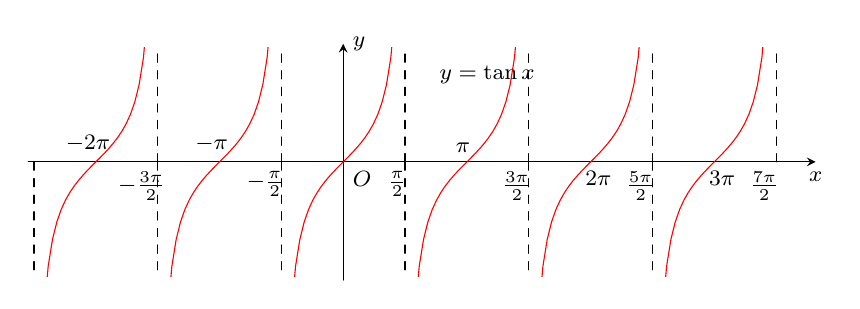
\begin{tikzpicture}[scale=0.5,>=stealth, font=\footnotesize, line join=round, line cap=round]
			\def\xmin{-8} \def\xmax{12} \def\ymin{-3} \def\ymax{3}
			\draw[->] (\xmin,0)--(\xmax,0) node [below]{$x$};
			\draw[->] (0,\ymin)--(0,\ymax) node [right]{$y$};
			\clip (\xmin+0.1,\ymin+0.1) rectangle (\xmax-0.5,\ymax-0.1);
			\node at (0,0) [below right]{$O$};
			\foreach \k in {-2,...,3} {
				\begin{scope}[xshift=pi*\k cm]
					\draw[red] plot[domain=-1.32:1.32] (\x,{tan(\x r)});
					\draw[dashed] (180:pi/2)--++(270:4) (0:pi/2)--++(90:4);
				\end{scope}
			}

			%	\draw[smooth,samples=200,domain=\xmin:\xmax] plot(\x,{tan(\x r)});
			\node at (-2*pi-0.2,0) [above]{$-2\pi$};
			\node at (-1.5*pi-0.4,0) [below]{$-\frac{3\pi}{2}$};
			\node at (-pi-0.2,0) [above]{$-\pi$};
			\node at (-0.5*pi-0.4,0) [below]{$-\frac{\pi}{2}$};
			\node at (0.5*pi-0.2,0) [below]{$\frac{\pi}{2}$};
			\node at (pi-0.1,0) [above]{$\pi$};
			\node at (1.5*pi-0.3,0) [below]{$\frac{3\pi}{2}$};
			\node at (2*pi+0.2,0) [below]{$2\pi$};
			\node at (2.5*pi-0.3,0) [below]{$\frac{5\pi}{2}$};
			\node at (3*pi+0.2,0) [below]{$3\pi$};
			\node at (3.5*pi-0.3,0) [below]{$\frac{7\pi}{2}$};
			\node at (1.1*pi+0.2,2.7) [below]{$y = \tan x$};
		\end{tikzpicture}
	\end{center}
	Tìm số giao điểm giữa đồ thị hàm số thuộc khoảng $\left(-\dfrac{5\pi}{2};\dfrac{7\pi}{2}\right)$ và đường thẳng $ y=\dfrac{2}{3} $.
	\choice
	{$4$}
	{$7$}
	{$5$}
	{\True $6$}
	\loigiai{
		Dựa vào đồ thị ta nhận thấy đồ thị hàm số $y=\tan x$ cắt đường thẳng $y=\dfrac{3}{2}$ tại $6$ điểm thuộc $\left(-\dfrac{5\pi}{2};\dfrac{7\pi}{2}\right)$.\\
		Vậy  có tất cả $6$ giao điểm.
	}
\end{ex}

\begin{ex}[Trích đề thi GHKI - Trường Trần Hưng Đạo - Nam Định - Năm học 2023-2024]%[1D1V4-6]%[Dự án đề cương 2025]%[Đoàn Minh Tâm]%Câu 10
	Cho số dương $a$. Gọi giá trị lớn nhất và giá trị nhỏ nhất của hàm số $y=1-\sqrt{a \cdot \cos^2x+1}$ lần lượt là $M$ và $m$. Giá trị của $M-m$ bằng
	\choice
	{$\sqrt{a+1}$}
	{$-\sqrt{a+1}$}
	{$1+\sqrt{a+1}$}
	{\True $-1+\sqrt{a+1}$}
	\loigiai{
		Với mọi $x \in \mathbb{R}$, ta có \allowdisplaybreaks
		\begin{eqnarray*}
			& &0 \leq \cos^2x \leq 1 \\
			&\Rightarrow &1 \leq a\cos^2x+1 \leq a+1\\
			&\Rightarrow &1 \leq \sqrt{a\cos^2x+1} \leq \sqrt{a+1}\\
			&\Rightarrow &-1 \geq -\sqrt{a\cos^2x+1} \geq -\sqrt{a+1}\\
			&\Rightarrow &0 \geq 1-\sqrt{a\cos^2x+1} \geq 1-\sqrt{a+1}\\
			&\Rightarrow &0 \geq y \geq 1-\sqrt{a+1}.
		\end{eqnarray*}
		Ngoài ra $y=0$ khi $\cos x=0 \Leftrightarrow x=\dfrac{\pi}{2}+k\pi$, $k \in \mathbb{Z}$.\\
		Và $y=1-\sqrt{a+1}$ khi $\cos^2x=1 \Leftrightarrow \sin x=0 \Leftrightarrow x=k\pi$, $k \in \mathbb{Z}$.\\
		Vậy $M=\max y=0$ và $m=\min y=1-\sqrt{a+1}$. Suy ra $M-m=-1+\sqrt{a+1}$.
	}
\end{ex}

\begin{ex}[Trích đề thi GHKI - Trường Thường Tín - Hà Nội - Năm học 2023-2024]%[1D1V4-8]%[Dự án đề cương 2025]%[Đoàn Minh Tâm]%Câu 10
	\immini{Một chất điểm chuyển động theo chiều ngược chiều kim đồng hồ trên đường tròn bán kính $5$ cm. Khoảng cách $h$ cm từ chất điểm đến trục hoành được tính theo công thức $h = |y|$, trong đó $y = 5 \sin\left(\dfrac{\pi}{5}t\right)$ với $t$ là thời gian chuyển động của chất điểm tính bằng giây $(t \geq 0)$ và chất điểm bắt đầu chuyển động từ vị trí A. Khi $t=\dfrac{5}{6}$ giây thì khoảng cách $h$ bằng}
	{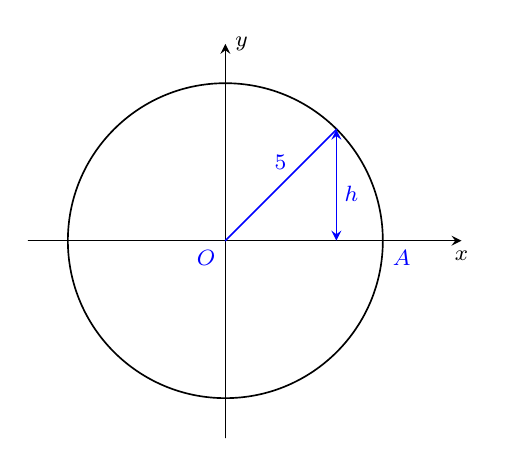
\begin{tikzpicture}[line join=round,line cap=round,line width=.6pt,font=\footnotesize,scale=1]
			\draw[-stealth] (-2.5,0) -- (3,0)node[below] {$x$};
			\draw[-stealth] (0,-2.5) -- (0,2.5)node[right] {$y$};
			\def\a{1}
			\draw[black] (0,0) circle (2);
			\draw[blue] (0:0) node[below left]{$O$}--(45:2);
			\draw[stealth-stealth, blue] (1.41,0)--(1.41,1.41);
			\path (0:2) node[below right,blue]{$A$};
			\path (0.7,1) node[blue]{$5$};
			\path (1.6,0.6) node[blue]{$h$};
	\end{tikzpicture}}
	\choice
	{$h=0{,}5$ cm}
	{$h=5$ cm}
	{$h=2$ cm}
	{\True $h=2{,}5$ cm}
	\loigiai
	{Khoảng cách $h$ được xác định bởi $h = |y|=\left| 5 \sin\left(\dfrac{\pi}{5}t\right)\right|$.\\
		Khi $t=\dfrac{5}{6}$ giây thì khoảng cách $h = |y|=\left| 5 \sin\left(\dfrac{\pi}{5}\cdot \dfrac{5}{6}\right)\right|=\dfrac{5}{2}=2{,}5$ (cm).
	}
\end{ex}
\Closesolutionfile{ans}

\ind{PHẦN II.} \inden{Câu trắc nghiệm đúng sai. Trong mỗi ý a), b), c), d) ở mỗi câu, học sinh chọn đúng hoặc sai.}\\
\setcounter{ex}{0}
\Opensolutionfile{ans}[ans/1D1-Bai3-DS]%--Đặt tên 2D1-Bai1-DS
\begin{ex}[Trích đề thi GHKI - Trường Chuyên Bình Thuận - Năm học 2024-2025]%[1D1H4-4]%[Dự án đề cương 2025]%[Đoàn Minh Tâm]%Câu 1
	Cho hàm số $f(x)=\tan x-x$. Khi đó
	\choiceTF
	{\True Tập xác định của hàm số là $\mathscr{D}=\mathbb{R}\setminus \left\{\dfrac{\pi}{2}+k\pi,\, k\in \mathbb{Z}\right\}$}
	{$f\left(\dfrac{\pi}{3} \right)=f\left(-\dfrac{\pi}{3} \right)$}
	{\True $f\left(-x\right)=-f(x)$, $\forall x\in \mathbb{R}$}
	{Đồ thị hàm số nhận trục $Oy$ làm trục đối xứng}
	\loigiai{
		\begin{itemchoice}
			\itemch
			Hàm số $f(x)=\tan x$ có điều kiện xác định là $x\ne \dfrac{\pi}{2}+k\pi$, $k\in \mathbb{Z}$.
			\itemch
			Ta có
			\begin{itemize}
				\item $f\left(\dfrac{\pi}{3} \right)= \sqrt{3}-\dfrac{\pi}{3}$,
				\item $f\left(-\dfrac{\pi}{3} \right)= -\sqrt{3}+\dfrac{\pi}{3}$.
			\end{itemize}
			Suy ra $f\left(\dfrac{\pi}{3} \right)\ne f\left(-\dfrac{\pi}{3} \right)$.
			\itemch
			Ta có $f(-x)= \tan (-x) +x=-\tan x +x=-(\tan x -x)=-f(x)$, $\forall x\in \mathbb{R}$.
			\itemch
			Ta có $f\left(-x\right)=-f(x)$ nên hàm số $f(x)$ là hàm số lẻ.\\
			Vậy đồ thị của hàm số nhận gốc tọa độ $O$ làm tâm đối xứng.
		\end{itemchoice}
	}
\end{ex}

\begin{ex}[Trích đề thi GHKI - Trường Trần Phú - Năm học 2024-2025]%[1D1V4-4]%[Dự án đề cương 2025]%[Đoàn Minh Tâm]%Câu 2
	Cho hàm số $f(x)=\dfrac{10}{3\cos x+5}$.
	\choiceTF
	{\True Hàm số $f(x)$ có tập xác định là tập số thực $\mathbb{R}$}
	{Hàm số $f(x)$ là hàm số lẻ trên $\mathbb{R}$}
	{\True Giá trị lớn nhất của hàm số $f(x)$ trên $\left[-\dfrac{\pi}{2} ; \dfrac{\pi}{2}\right]$ bằng $2$}
	{Nếu $f(x)=3$ thì $\cos 2x=\dfrac{31}{81}$}
	\loigiai{
		\begin{itemchoice}
			\itemch  Ta có $3\cos x+5\neq 0$ với mọi $x$.\\
			Vậy hàm số $f(x)$ có tập xác định là tập số thực $\mathbb{R}$.
			\itemch  $\forall x\in \mathbb{R}, -x\in\mathbb{R}$, khi đó ta có $f(-x)=\dfrac{10}{3\cos(-x)+5}=\dfrac{10}{3\cos x+5}=f(x)$.\\
			Vậy $f(x)$ là hàm số chẵn.
			\itemch  Vì $x\in \left[-\dfrac{\pi}{2} ; \dfrac{\pi}{2}\right]$ nên $ 0\leq\cos x\leq1$ suy ra $ 0\leq3\cos x\leq3$.\\
			Từ đó suy ra $5\leq 3\cos(x)+5\leq 8$. Do đó $\dfrac{10}{8}\leq f(x)\leq 2$.\\Vậy giá trị lớn nhất của hàm số $f(x)$ trên $\left[-\dfrac{\pi}{2} ; \dfrac{\pi}{2}\right]$ bằng $2$.
			\itemch Ta có
			\begin{eqnarray*}
				&&f(x)=3\\
				&\Rightarrow& \dfrac{10}{3\cos x+5}=3\\
				&\Rightarrow& 3\cos x+5=\dfrac{10}{3}\\
				&\Rightarrow& \cos x=-\dfrac{5}{9}\\
				&\Rightarrow& \cos 2x=2\cos^{2}x-1=2\cdot\left(-\dfrac{5}{9} \right)^2-1=- \dfrac{31}{81}.
			\end{eqnarray*}
		\end{itemchoice}
	}
\end{ex}

\begin{ex}%[1D1H4-7]%[Dự án đề cương 2025]%[Đoàn Minh Tâm]%Câu 3
	Cho hàm số $y=\cos x$.
	\choiceTF
	{Tập xác định của hàm số $\mathbb{R}$ và tập giá trị của hàm số là $T=\left[0;1\right]$}
	{\True Đồ thị hàm số đi qua điểm $\left(\dfrac{\pi}{4}; \dfrac{\sqrt{2}}{2} \right)$}
	{\True Đồ thị hàm số $y=\sin x$ cắt trục hoành tại vô số điểm}
	{Đồ thị hàm số $y=\cos x$ không cắt đường thẳng $y=2m+3$ (với $m\in \mathbb{R}$ là tham số) khi $m < -\dfrac{3}{2}$}
	\loigiai{
		\begin{itemchoice}
			\itemch Xét hàm số $y=\cos x$ có\\
			Tập xác định là $\mathscr{D}=\mathbb{R}$.
			Tập giá trị của hàm số là $T=\left[-1;1\right]$.
			\itemch Hàm số $y=\cos x$.\\
			Với $x=\dfrac{\pi}{4}$ ta có $y=\cos x=\sin \dfrac{\pi}{4}=\dfrac{\sqrt{2}}{2}$
			\itemch Đồ thị hàm số $y=\cos x$ cắt trục hoành tại vô số điểm.\\
			Hàm số $y=\cos x$ và trục hoành $y=0$.\\
			Phương trình hoành độ số giao điểm của hai đồ thị là: $\cos x=0\Leftrightarrow x=\dfrac{\pi}{2}+k\pi \left(k\in \mathbb{Z}\right)$.\\
			Với mỗi giá trị $k\in \mathbb{R}$ ta được một nghiệm tức là một giao điểm do đó
			phương trình trên có vô số nghiệm.\\
			Vậy đồ thị hàm số $y=\cos x$ cắt trục hoành tại vô số điểm.
			\itemch Phương trình hoành độ giao điểm đồ thị hàm số $y=\cos x$ và đường thẳng $y=2m+3$ là $\cos x=2m+3$.\\
			Đồ thị hàm số $y=\cos x$ không cắt đường thẳng $y=2m+3$ (với $m\in \mathbb{R}$ là tham số) khi phương trình $\cos x=2m+3$ vô nghiệm.\\
			Vậy ta có $\hoac{&2m+3> 1\\&2m+3<-1}\Leftrightarrow \hoac{&m >-1\\&m <-2}\Leftrightarrow m\in \left(-\infty;-2\right)\cup \left(-1;-\infty \right)$.
		\end{itemchoice}
	}
\end{ex}

\begin{ex}[Trích đề thi GHKI - Trường Tây Thạnh - Năm học 2024-2025]%[1D1V5-6]%[Dự án đề cương 2025]%[Đoàn Minh Tâm]%Câu 3
	Giả sử nhiệt độ bên trong một ngôi nhà sau $t$ (giờ) kể từ $12$ giờ trưa, gọi là $T(t)$ được tính bởi $T(t)=5\cos\left(\dfrac{\pi}{2}-\dfrac{\pi t}{6}\right)+25$ ($^\circ$C) với $0\leq t \leq 24$.
	\choiceTF
	{$T(0)=29$}
	{\True $T(12)=T(6)$}
	{Nhiệt độ cao nhất trong ngôi nhà là $36^\circ$C}
	{\True Nhiệt độ trong ngôi nhà lúc $5$ giờ chiều là $27{,}5^\circ$C}
	\loigiai{
		\begin{itemchoice}
			\itemch Ta có $T(0)=25$.
			\itemch Ta có $T(12)=25$ và $T(6)=25$. Vậy $T(12)=T(6)$.
			\itemch	Do $-1\leq \cos\left(\dfrac{\pi}{2}-\dfrac{\pi t}{6}\right) \leq 1$ nên $20\leq 5\cos\left(\dfrac{\pi}{2}-\dfrac{\pi t}{6}\right)+25 \leq 30$.\\\
			Suy ra nhiệt độ cao nhất trong ngôi nhà là $30^\circ$C khi $\cos\left(\dfrac{\pi}{2}-\dfrac{\pi t}{6}\right)=1$ hay $t=3$, $t=15$.
			\itemch Lúc $5$ giờ chiều, tức sau $12$ giờ trưa là $5$ giờ, suy ra $t=5$.\\
			Ta có $T(5)=27{,}5^\circ$C.
		\end{itemchoice}
	}
\end{ex}

\begin{ex}[Trích đề thi GHKI - Trường Nguyễn Thị Minh Khai - Năm học 2024-2025]%[1D1V5-6]%[Dự án đề cương 2025]%[Đoàn Minh Tâm]%Câu 4
	Huyết áp là áp lực máu cần thiết tác động lên thành động mạch nhằm đưa máu đi nuôi dưỡng các mô trong cơ thể. Nhờ lực co bóp của tim và sức cản của động mạch mà huyết áp được tạo ra. Giả sử huyết áp của một người thay đổi theo thời gian được cho bởi công thức: $p(t)=120+15 \cos 150 \pi t$, trong đó $p(t)$ là huyết áp tính theo đơn vị mmHg (milimét thuỷ ngân) và thời gian $t$ tính theo đơn vị phút. Huyết áp cao nhất được gọi là huyết áp tâm thu và huyết áp thấp nhất được gọi là huyết áp tâm trương.
	\choiceTF
	{\True $-1 \leq \cos 150 \pi t \leq 1, \forall t \geq 0$}
	{$p(2)=120 \mathrm{mmHg}$}
	{\True Huyết áp tâm thu của người đó là $135$ mmHg và huyết áp tâm trương của người đó là $105$ mmHg}
	{Trong thời gian từ $0$ giây đến $30$ giây, huyết áp của một người có $75$ lần đạt $120$ mmHg}
	\loigiai{
		\begin{itemchoice}
			\itemch Vì $-1 \leq \cos 150 \pi t \leq 1, \forall t \geq 0$.
			\itemch Thay $t=2$ vào biểu thức $p(t)=120+15 \cos 150 \pi t$, \\
			ta được $p(2)=120+15 \cos (150 \cdot \pi \cdot 2)=135$ mmHg.
			\itemch Ta có
			\begin{eqnarray*}
				&&-1 \leq \cos 150 \pi t \leq 1 \\&\Leftrightarrow& -15 \leq 15 \cos 150 \pi t \leq 15\\ &\Leftrightarrow& 105 \leq 120 + 15 \cos 150 \pi t \leq 135
			\end{eqnarray*}
			Vậy huyết áp tâm thu của người đó là $135$ mmHg, huyết áp tâm trương là $105$ mmHg.
			\itemch Vì huyết áp của một người đạt $120$ mmHg nên \begin{eqnarray*}
				&& 120 + 15 \cos 150 \pi t = 120 \\&\Leftrightarrow& \cos 150 \pi t =0 \\&\Leftrightarrow & 150 \pi t=\dfrac{\pi}{2}+k \pi\\
				&\Leftrightarrow& t=\dfrac{1}{300}+\dfrac{1}{150}k.
			\end{eqnarray*}
			Xét thời gian từ $0$ giây đến $30$ giây, ta có
			\begin{eqnarray*}
				&&0\leq t \leq 30 \\
				&\Leftrightarrow& 0 \leq \dfrac{1}{300}+\dfrac{1}{150}k \leq 30\\ &\Leftrightarrow& -\dfrac{1}{300} \leq \dfrac{1}{150}k \leq \dfrac{8\,999}{300}\\ &\Leftrightarrow& -\dfrac{1}{4} \leq k \leq \dfrac{8\,999}{2}.
			\end{eqnarray*}
			Vì $k \in \mathbb{Z}$ nên $k \in \{0;1;2; \ldots ;4499\}$.\\
			Vậy có $4\,450$ lần huyết áp đạt $120$ mhHg.
		\end{itemchoice}
	}
\end{ex}


\Closesolutionfile{ans}

\ind{PHẦN III.} \inden{Câu trả lời ngắn.}\\
\setcounter{ex}{0}
\Opensolutionfile{ans}[ans/1D1-Bai3-TLN]%--Đặt tên 2D1-Bai1-DS
\begin{ex}%[1D1H4-6]%[Dự án đề cương 2025]%[Đoàn Minh Tâm]%Câu 1
	Tìm tổng bình phương giá trị lớn nhất và giá trị nhỏ nhất của hàm số $y=\sin x+\cos x$. \shortans{$4$}
	\loigiai{
		$$y=\sin x+\cos x=\sqrt{2} \sin x\cdot \cos \dfrac{\pi}{4}+\sqrt{2} \cos x\cdot \sin \dfrac{\pi}{4}=\sqrt{2} \sin \left(x+\dfrac{\pi}{4} \right).$$
		$-1\le \sin \left(x+\dfrac{\pi}{4} \right)\le 1,\, \forall x\Leftrightarrow-\sqrt{2} \le y\le \sqrt{2}$. Suy ra $y_{min\;}=-\sqrt{2}$ và $y_{\max}=\sqrt{2}$.\\
		Do đó $y_{min}^2+y_{\max}^2=4$.
	}
\end{ex}

\begin{ex}[Trích đề thi GHKI - Trường Chuyên Bình Thuận - Năm học 2024-2025]%[1D1V4-8]%[Dự án đề cương 2025]%[Đoàn Minh Tâm]%Câu 2
	Hằng ngày mực nước tại một bến cảng lên xuống theo thủy triều. Độ sâu $h$ (m) của mực nước theo thời gian $t$ (giờ) trong một ngày được cho bởi công thức:
	$$h(t)=11+2\sin\left(\dfrac{\pi}{12}t\right),$$
	với $0\le t\le 24$. Mực nước thấp nhất tại cảng là bao nhiêu?
	\shortans[oly]{$ 13 $}
	\loigiai{
		Với mọi $t$, ta có $-1\le \sin\left(\dfrac{\pi}{12}t\right)\le 1$. Suy ra
		$$9\le 11+2\sin\left(\dfrac{\pi}{12}t\right) \le 13.$$
		Vậy mực nước thấp nhất tại cảng là $13$ m.
	}
\end{ex}

\begin{ex}[Trích đề thi GHKI - Trường Nguyễn An Ninh - Năm học 2024-2025]%[1D1H4-8]%[Dự án đề cương 2025]%[Đoàn Minh Tâm]%Câu 2
	Độ sâu $D(t)$ m của nước ở một cảng biển sau $t$ giờ kể từ lúc nữa đêm được tính bởi công thức $D(t) = 4 \cos \left( \dfrac{\pi t}{6} \right) + 6$  (m); $(0\le t\le 24)$. Độ sâu của nước ở cảng này sau $14$ giờ là bao nhiêu mét?
	\shortans[oly]{$8$}
	\loigiai{
		Dựa vào công thức đã cho
		\[ D(t) = 4 \cos \left( \frac{\pi t}{6} \right) + 6  \text{ (m)}. \]
		Tính độ sâu của nước tại thời điểm $t = 14$ giờ.\\
		Thay $t = 14$ vào công thức
		\[
		D(14) = 4 \cos \left( \frac{\pi \cdot 14}{6} \right) + 6=8.
		\]
		Độ sâu của nước ở cảng này lúc $14$ giờ là $8$ mét.

	}
\end{ex}

\begin{ex}[Trích đề thi GHKI - Trường Nguyễn Bỉnh Khiêm - Hà Nội - Năm học 2024-2025]%[1D1H4-6]%[Dự án đề cương 2025]%[Đoàn Minh Tâm]%Câu 4
	Giả sử hàm số $y=\sin (2\,024x + 1) - 2$ có giá trị lớn nhất và giá trị nhỏ nhất lần lượt là $M$, $m$. Tìm $M-3m$.
	\shortans[oly]{$ 8 $}
	\loigiai{Xét hàm số $y=\sin (2\,024x + 1) - 2$.\\
		Tập xác định $\mathscr{D}=\mathbb{R}$.\\
		Với mọi $x\in\mathscr{D}$, ta có
		\begin{eqnarray*}
			& &-1\leq \sin(2\,024x+1)\leq 1\\
			&\Leftrightarrow &-3 \leq \sin (2\,024x+1) \leq -1\\
			&\Leftrightarrow &-3 \leq y \leq -1.
		\end{eqnarray*}
		Ta có $\max\limits_{\mathscr{D}}y=-1$ khi $\sin (2\,024x+1) = 1 \Leftrightarrow x= \dfrac{\pi -2}{4\,048} + \dfrac{k\pi}{1\, 012} $. Suy ra $M=-1$.\\
		Ta có $\min\limits_{\mathscr{D}}y =-3$ khi $\sin (2\, 024 x + 1)=-1 \Leftrightarrow x=- \dfrac{\pi+2}{4\,048} + \dfrac{k\pi}{1\,012}$. Suy ra $m=-3$.\\
		Khi đó $M-3m=8$.
	}
\end{ex}

\begin{ex}%[1D1C4-8]%[Dự án đề cương 2025]%[Đoàn Minh Tâm]%Câu 5
	Một cây cầu có dạng cung $OA$ là một phần của đồ thị hàm số $y=4{,}8 \sin \dfrac{x}{9}$ và được mô tả trong hệ trục tọa độ với đơn vị trục là mét như hình bên.
	\begin{center}
		\begin{tikzpicture}%[line join=round, line cap=round,>=stealth,scale=.85,transform shape]
			\def\xmin{0} 	\def\xmax{12}	\def\ymin{-.5} \def\ymax{2}
			\draw[->](\xmin-.5,0)--(\xmax+1,0) node[below]{$x$};
			\draw[->](0,\ymin)--(0,\ymax+.5) node[left]{$y$};
			\draw (0,0) node[below right]{$O$};
			\draw[red, thick] (\xmin,0) to [out=40, in= 140] (\xmax,0)node[below]{$A$};
		\end{tikzpicture}
	\end{center}
	Giả sử chiều rộng của con sông là độ dài đoạn thẳng $OA$. Chiều rộng đó (làm tròn đến kết quả hàng phần mười) là
	\shortans{$28{,}3$}
	\loigiai{
		Phương trình hoành độ giao điểm
		$$4{,}8 \sin \dfrac{x}{9}=0\Leftrightarrow\sin \dfrac{x}{9}=0\Leftrightarrow\dfrac{x}{9}=k\pi\Leftrightarrow x=9k\pi,\ (k\in \mathbb{Z}).$$
		Hoành độ điểm $A$ ứng với $x=9\pi$.\\
		Vậy $OA=9\pi\approx 28{,}3$m.
	}
\end{ex}


\Closesolutionfile{ans}

\ind{PHẦN IV.} \inden{Tự luận.}\\
\setcounter{ex}{0}
\begin{ex}[Trích đề thi GHKI - Trường Nguyễn Chí Thanh - Năm học 2023-2024]%[1D1N4-2]%[Dự án đề cương 2025]%[Đoàn Minh Tâm]%Câu 1
	Tìm tập xác định của hàm số $y=\cot \left(2 x-\dfrac{\pi}{3}\right)$.
	\loigiai{Điều kiện xác định $2 x-\dfrac{\pi}{3} \ne k\pi \Leftrightarrow x \ne \dfrac{\pi}{6}+k\dfrac{\pi}{2}$ ($k\in \mathbb{Z}$).\\
		Vậy tập xác định là $\mathscr{D}=\mathbb{R}\setminus\left\lbrace \dfrac{\pi}{6}+k\dfrac{\pi}{2} \mid k \in \mathbb{Z} \right\rbrace$.
	}
\end{ex}

\begin{ex}[Trích đề thi GHKI - Trường Tenloman - Năm học 2023-2024]%[1D1N4-8]%[Dự án đề cương 2025]%[Đoàn Minh Tâm]%Câu 1
	Nếu độ cao của mực nước thủy triều được tính theo công thức $h(t)=4+2\cos \left(\dfrac{\pi t}{12}+\dfrac{3\pi}{2}\right)$ với $ t $ là thời gian trong ngày tính theo giờ và độ cao mực nước tính theo đơn vị m. Tính độ cao của mực nước vào lúc $ 6 $ giờ sáng.
	\loigiai{Ta có $h(6)=4+2\cos \left(\dfrac{\pi \cdot 6 }{12}+\dfrac{3\pi}{2}\right)=6$ m.
	}
\end{ex}

\begin{ex}[Trích đề thi GHKI - Trường Bà Điểm - Năm học 2023-2024]%[1D1V4-2]%[Dự án đề cương 2025]%[Đoàn Minh Tâm]%Câu 2
	Tìm tập xác định của hàm số $y=\dfrac{\cot 2x}{2\sin x-1}$.
	\loigiai{Hàm số $y=\dfrac{\cot 2x}{2\sin x-1}$
		xác định khi
		\[\heva{&2\sin x -1 \neq 0\\&\sin 2x \neq 0}\Leftrightarrow \heva{& x \neq \dfrac{\pi}{6}+k2\pi\\& x\neq \dfrac{5\pi}{6}+k2\pi\\& 2x \neq k\pi}\Leftrightarrow \heva{& x \neq \dfrac{\pi}{6}+k2\pi\\& x\neq \dfrac{5\pi}{6}+k2\pi\\& x \neq \dfrac{k\pi}{2}}, \  \ k \in \mathbb{Z}.\]
		Vậy tập xác định của hàm số đã cho là $\mathscr{D}=\mathbb{R} \setminus \left\{\dfrac{\pi}{6}+k2\pi, \ \dfrac{5\pi}{6}+k2\pi, \  \dfrac{k\pi}{2}\  \text{với } \ k \in \mathbb{Z}\right\}$.

	}
\end{ex}

\begin{ex}[Trích đề thi GHKI - Trường Phạm Phú Thứ - Năm học 2023-2024]%[1D1H4-2]%[Dự án đề cương 2025]%[Đoàn Minh Tâm]%Câu 3
	Tìm tập xác định của các hàm số sau
	\begin{multicols}{2}
		\begin{enumerate}
			\item $y=\sin x+\tan \left(x+\dfrac{\pi}{3}\right)$;
			\item $y=\dfrac{\cos x}{1-\sin 4 x}$.
		\end{enumerate}
	\end{multicols}
	\loigiai{
		\begin{enumerate}
			\item Hàm số xác định khi
			$$x+\dfrac{\pi}{3} \ne \dfrac{\pi}{2} + k\pi  \Leftrightarrow x \ne \dfrac{\pi}{6} +k\pi \quad \left( k \in \mathbb{Z} \right). $$
			Vậy tập xác định của hàm số là $\mathscr{D}= \mathbb{R} \setminus \left\{ \dfrac{\pi}{6} +k\pi \mid k \in \mathbb{Z}  \right\}$.
			\item  Hàm số xác định khi
			$$ 1- \sin4x \ne 0 \Leftrightarrow 4x \ne \dfrac{\pi}{2} +k2\pi \Leftrightarrow x \ne \dfrac{\pi}{8} + \dfrac{k\pi}{2} \quad  \left( k \in \mathbb{Z} \right). $$
			Vậy tập xác định của hàm số là $\mathscr{D}= \mathbb{R} \setminus \left\{ \dfrac{\pi}{8} +\dfrac{k\pi}{2} \mid k \in \mathbb{Z}   \right\}$.
		\end{enumerate}
	}
\end{ex}

\begin{ex}[Trích đề thi GHKI - Trường Phạm Phú Thứ - Năm học 2023-2024]%[1D1H4-3]%[Dự án đề cương 2025]%[Đoàn Minh Tâm]%Câu 3
	Tìm tập giá trị của hàm số $y = 2\cos^2 x + 5$ trên $\mathbb{R}$.
	\loigiai{
		Ta có $0\leq \cos^2 x \leq 1 \Leftrightarrow 0\leq 2\cos^2x \leq 2 \Leftrightarrow 5\leq 2\cos^2x + 5 \leq 6\Leftrightarrow 5\leq y \leq 7$.
		\\Vậy tập giá trị của hàm số là $\left[5; 7\right]$.
	}
\end{ex}

\begin{ex}[Trích đề thi GHKI - Trường Tenloman - Năm học 2023-2024]%[1D1H4-3]%[Dự án đề cương 2025]%[Đoàn Minh Tâm]%Câu 4
	\begin{enumerate}
		\item Cho $\cos a=\dfrac{1}{3}$. Tính giá trị của biểu thức $A=2-2 \cdot \sin ^2 a$.
		\item Cho $\sin a=\dfrac{4}{5}\left(\dfrac{\pi}{2}<a<\pi\right)$. Tính giá trị lượng giác $\cos \left(\dfrac{\pi}{6}+a\right)$.
		\item Tìm tập giá trị của hàm số $y=4 \cdot \sin 2 x+1$ trên tập hợp các số thực $\mathbb{R}$.
	\end{enumerate}
	\loigiai{
		\begin{enumerate}
			\item  $  \sin ^2 a=1-\left(\dfrac{1}{3}\right)^2=\dfrac{8}{9}$.\\
			Suy ra $A=2 \cos ^2 a=2 \cdot\left(\dfrac{1}{3}\right)^2=\dfrac{2}{9}$.
			\item $	 \cos a=\dfrac{-3}{5} $.
			Ta có $\cos \left(\dfrac{\pi}{6}+a\right)=\dfrac{-3}{5} \cdot \dfrac{\sqrt{3}}{2}-\dfrac{4}{5} \cdot \dfrac{1}{2}=-\dfrac{3 \sqrt{3}+4}{10}$.
			\item $	 -1 \leq \sin 2 x \leq 1 \Leftrightarrow
			-3 \leq y \leq 5 $.\\
			Vậy $T=\left[-3;5\right]$.
		\end{enumerate}
	}
\end{ex}


\begin{ex}[Trích đề thi GHKI - Trường Trần Khai Nguyên - Năm học 2023-2024]%[1D1V4-8]%[Dự án đề cương 2025]%[Đoàn Minh Tâm]%Câu 5
	Chiều cao $h$ mét của một cabin trên vòng quay vào thời điểm $t$ giây sau khi bắt đầu chuyển động được cho bởi công thức $h(t)=25+20\sin\left(\dfrac{\pi}{30}t+\dfrac{\pi}{3}\right)$.
	\begin{enumerate}
		\item Cabin đạt độ cao bao nhiêu khi bắt đầu chuyển động và sau khi chuyển động được $30$ giây.
		\item Tìm những thời điểm trong $2{,}5$ phút đầu tiên mà cabin đạt độ cao $45$ m.
	\end{enumerate}
	\loigiai{
		\begin{enumerate}
			\item Ta có
			\begin{itemize}
				\item $h(0)=25+20\sin\left(\dfrac{\pi}{3}\right)=25+10\sqrt{3}$ m.
				\item $h(30)=25+20\sin\left(\dfrac{\pi}{30}\cdot 30+\dfrac{\pi}{3}\right)=25-10\sqrt{3}$ m.
			\end{itemize}
			\item Xét phương trình\\
			\allowdisplaybreaks
			\begin{eqnarray*}
				& &25+20\sin\left(\dfrac{\pi}{30}t+\dfrac{\pi}{3}\right)=45\\ &\Leftrightarrow &20\sin\left(\dfrac{\pi}{30}t+\dfrac{\pi}{3}\right)=20\\
				&\Leftrightarrow &\sin\left(\dfrac{\pi}{30}t+\dfrac{\pi}{3}\right)=1\\ &\Leftrightarrow &\dfrac{\pi}{30}t+\dfrac{\pi}{3}=\dfrac{\pi}{2}+k2\pi\\
				&\Leftrightarrow &t=5+60k, \quad (k\in\mathbb{Z}).
			\end{eqnarray*}
			Có $0\le 5+60k\le 150 \Leftrightarrow -\dfrac{5}{60}\le k\le \dfrac{145}{60}$.\\
			Mà $k\in\mathbb{Z}$ suy ra $k\in \{1;2\}$.\\
			Vậy trong $2{,}5$ phút đầu tiên cabin đạt độ cao $45$ m tại $t_1=65$ giây và $t_2=125$ giây.
		\end{enumerate}}
\end{ex}

\begin{ex}[Trích đề thi GHKI - Trường Trần Hưng Đạo - Năm học 2023-2024]%[1D1V4-8]%[Dự án đề cương 2025]%[Đoàn Minh Tâm]%Câu 5
	Nhiệt độ ngoài trời ở một thành phố vào các thời điểm khác nhau trong ngày có thể được mô phỏng bởi công thức $f(t)=29 + 8\cos\left[\dfrac{\pi}{4}\left( 4-\dfrac{t}{3}\right) \right]$, với $f$ tính bằng độ C và $t$ tính bằng giờ ($0\leq t \leq 24$).
	\begin{enumerate}
		\item Nhiệt độ cao nhất trong ngày là bao nhiêu độ C và vào lúc mấy giờ?
		\item Các công nhân công ty môi trường muốn cắt tỉa các cây trồng ở dải phân cách hai làn đường, họ bắt đầu làm việc từ $6$ giờ và kết thúc lúc $17$ giờ trong ngày. Dựa vào đồ thị hàm số côsin (xem hình bên dưới), hãy cho biết họ nên làm việc vào những thời điểm nào trong ngày để tránh nhiệt độ trên $36^\circ$C (kết quả làm tròn đến hàng phần mười).
		\begin{center}
			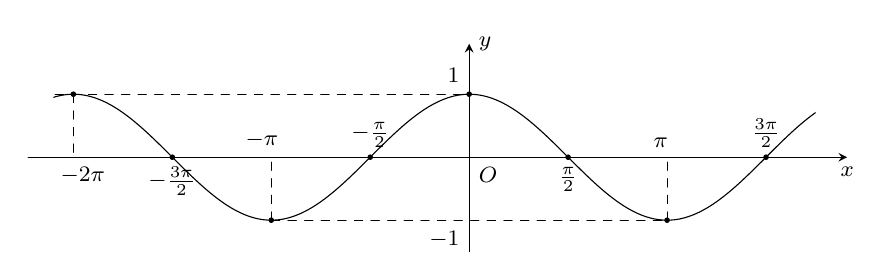
\begin{tikzpicture}[scale=0.8,>=stealth, font=\footnotesize, line join=round, line cap=round]
				\def\xmin{-10} \def\xmax{10.5} \def\ymin{-1.5} \def\ymax{1.8}
				\draw[->] (-7,0)--(6,0) node [below]{$x$};
				\draw[->] (0,\ymin)--(0,\ymax) node [right]{$y$};
				\node at (0,0) [below right]{$O$};
				\clip (\xmin+3.4,\ymin+0.1) rectangle (\xmax-5,\ymax-0.1);
				\draw[smooth,samples=400,domain=\xmin:\xmax] plot(\x,{cos(\x r)});
				\draw[dashed] (\xmin,1)--(0,1) (-3.14,-1)--(3.14,-1);
				\foreach \x in {-2*pi,-1.5*pi,-pi,-0.5*pi,0}
				{\draw[fill=black] (\x,cos \x*180/pi) circle (1pt);
					\draw[dashed] (\x,cos \x*180/pi)--(\x,0);
					\draw[fill=black] (-\x,cos -\x*180/pi) circle (1pt);
					\draw[dashed] (-\x,cos \x*180/pi)--(-\x,0);}
				\node at (0,1.3) [left]{$1$};
				\node at (0,-1.3) [left]{$-1$};
				\node at (-2*pi+0.15,0) [below]{$-2\pi$};
				\node at (-1.5*pi,0) [below]{$-\frac{3\pi}{2}$};
				\node at (-pi-0.15,0) [above]{$-\pi$};
				\node at (-0.5*pi,0) [above]{$-\frac{\pi}{2}$};
				\node at (0.5*pi,0) [below]{$\frac{\pi}{2}$};
				\node at (pi-0.1,0) [above]{$\pi$};
				\node at (1.5*pi,0) [above]{$\frac{3\pi}{2}$};
			\end{tikzpicture}
		\end{center}
	\end{enumerate}

	\loigiai{
		\begin{enumerate}
			\item Ta có
			\begin{eqnarray*}
				&-1&\leq \cos\left[\dfrac{\pi}{4}\left( 4-\dfrac{t}{3}\right) \right]\leq 1\\ &\Leftrightarrow& - 8 \leq  8\cos\left[\dfrac{\pi}{4}\left( 4-\dfrac{t}{3}\right) \right]\leq 8\\ &\Leftrightarrow& 21 \leq 29 + 8\cos\left[\dfrac{\pi}{4}\left( 4-\dfrac{t}{3}\right) \right] \leq 37\\
				&\Leftrightarrow& 21 \leq f(t)\leq 37.
			\end{eqnarray*}
			$\max f(t) = 37$ khi $\cos\left[\dfrac{\pi}{4}\left( 4-\dfrac{t}{3}\right) \right] = 1\Leftrightarrow \dfrac{\pi}{4}\left( 4-\dfrac{t}{3}\right) = k2\pi \Leftrightarrow t = 3(4-8k)$.\\
			Do $0\leq t \leq 24$ cho nên $-\dfrac{1}{2}\leq k \leq \dfrac{1}{2}$ ta chọn $k = 0 \Rightarrow t = 12$.\\
			Vậy nhiệt độ cao nhất trong ngày là $37$ độ C vào lúc $12$ giờ.
			\item
			\begin{center}
				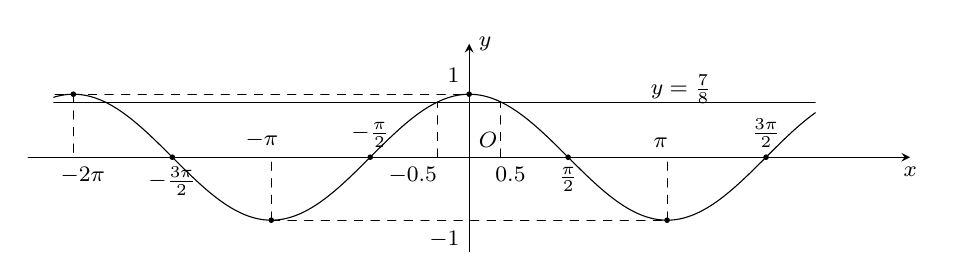
\begin{tikzpicture}[scale=0.8,>=stealth, font=\footnotesize, line join=round, line cap=round]
					\def\xmin{-10} \def\xmax{10.5} \def\ymin{-1.5} \def\ymax{1.8}
					\draw[->] (-7,0)--(7,0) node [below]{$x$};
					\draw[->] (0,\ymin)--(0,\ymax) node [right]{$y$};
					\node at (0,0) [above right]{$O$};
					\clip (\xmin+3.4,\ymin+0.1) rectangle (\xmax-5,\ymax-0.1);
					\draw[smooth,samples=400,domain=\xmin:\xmax] plot(\x,{cos(\x r)});
					\draw[dashed] (\xmin,1)--(0,1) (-3.14,-1)--(3.14,-1);
					\draw
					(\xmin,7/8)--(\xmax,7/8);
					\foreach \x in {-2*pi,-1.5*pi,-pi,-0.5*pi,0}
					{\draw[fill=black] (\x,cos \x*180/pi) circle (1pt);
						\draw[dashed] (\x,cos \x*180/pi)--(\x,0);
						\draw[fill=black] (-\x,cos -\x*180/pi) circle (1pt);
						\draw[dashed] (-\x,cos \x*180/pi)--(-\x,0);}
					\node at (0,1.3) [left]{$1$};
					\node at (0,-1.3) [left]{$-1$};
					\node at (-2*pi+0.15,0) [below]{$-2\pi$};
					\node at (0.161*pi+0.15,0) [below  ]{$0.5$};
					\node at (-0.161*pi+0.15,0) [below left ]{$-0.5$};
					\node at (4.0,0.7) [above left ]{$y = \frac{7}{8}$};
					\node at (-1.5*pi,0) [below]{$-\frac{3\pi}{2}$};
					\node at (-pi-0.15,0) [above]{$-\pi$};
					\node at (-0.5*pi,0) [above]{$-\frac{\pi}{2}$};
					\node at (0.5*pi,0) [below]{$\frac{\pi}{2}$};
					\node at (pi-0.1,0) [above]{$\pi$};
					\node at (1.5*pi,0) [above]{$\frac{3\pi}{2}$};
					\draw[dashed] (0.5,0)--(0.5,7/8);
					\draw[dashed] (-0.5,0)--(-0.5,7/8);
				\end{tikzpicture}
			\end{center}
			Theo đề bài ta có
			\begin{eqnarray*}
				&f(t)& \leq 36 \\&\Leftrightarrow& 29 + 8\cos\left[\dfrac{\pi}{4}\left( 4-\dfrac{t}{3}\right) \right] \leq 36\\ &\Leftrightarrow & \cos\left[\dfrac{\pi}{4}\left( 4-\dfrac{t}{3}\right) \right] \leq \dfrac{7}{8}\\& \Leftrightarrow& -0{,}5  \leq \dfrac{\pi}{4}\left( 4-\dfrac{t}{3}\right) \leq 0{,}5\\& \Leftrightarrow& 10{,}1 \leq t \leq 13{,}9.
			\end{eqnarray*}
		\end{enumerate}

		Như vậy để tránh nhiệt độ trên $36^\circ$C thì các công nhân làm việc từ $10{,1}$ giờ đến $13{,}9$ giờ.
	}
\end{ex}

\begin{ex}[Trích đề thi GHKI - Trường Thường Tín - Hà Nội - Năm học 2023-2024]%[1D1V6-8]%[Dự án đề cương 2025]%[Đoàn Minh Tâm]%Câu 5
	Độ sâu $h$ (m) của mực nước ở một cảng biến vào thời điểm $t$ (giờ) sau khi thủy triều lên lần đầu tiên trong ngày được tính xấp xỉ bởi công thức $h(t) = 0{,}8\cos t + 4$.\\
	Một con tàu cần mực nước sâu tối thiểu $3{,}6$ m để có thể di chuyển ra vào cảng an toàn. Dựa vào đồ thị của hàm số cô-sin, hãy cho biết trong vòng 6 giờ khi thủy triều lên lần đầu tiên, ở những thời điểm $t$ nào thì tàu có thể di chuyển ra vào cảng an toàn?
	\loigiai
	{
		Theo giả thiết, ta cần giải bất phương trình $h(t) \ge 3{,}6 \Leftrightarrow 0{,}8\cos t + 4\ge 3{,}6 \Leftrightarrow \cos t \ge -\dfrac{1}{2}$.
		\begin{center}
			\begin{tikzpicture}[scale=1, font=\footnotesize, line join=round, line cap=round, >=stealth]
				\draw[->] (-1,0) -- (8.5,0) node[above] {\small $x$};
				\draw[->] (0,-1.4) -- (0,1.8) node[right] {\small $y$};
				\draw[thick,blue,samples=100,domain=-1:7.5] plot(\x,{cos((\x)*180/pi)}) node[above right]{$y = \cos x$};
				\draw[dashed] (-1,1)--(7.5,1) (-1,-1)--(7.5,-1);
				\draw[thick,red] (-1,-0.5)--(7.5,-0.5) node[right]{$y=-\tfrac{1}{2}$};
				\draw[fill=black] (0,0) circle (1pt) node[above left]{$0$} (pi/2,0) circle (1pt) (pi,0) node[above]{$\pi$} circle (1pt) (3*pi/2,0) circle (1pt) (2*pi/2,0) circle (1pt) (6,0) node[below]{$6$} circle (1pt) (2*pi/3,0) node[above]{$\tfrac{2\pi}{3}$} circle (1pt) (4*pi/3,0) node[above]{$\tfrac{4\pi}{3}$} circle (1pt) (2*pi/3,-0.5) circle (1pt) (4*pi/3,-0.5) circle (1pt) (0,1) node[above left]{$1$} circle (1pt) (0,-1) node[below left]{$-1$} circle (1pt) (pi,-1) circle (1pt);
				\draw[dashed] (2*pi/3,0) -- (2*pi/3,-0.5) (4*pi/3,0) -- (4*pi/3,-0.5) (pi,0)--(pi,-1) (6,0)--(6,0.96);
			\end{tikzpicture}
		\end{center}
		Dựa vào đồ thị của hàm số cô-sin, ta thấy trong vòng 6 giờ khi thủy triều lên lần đầu tiên, ở những thời điểm $t$ thỏa mãn $0\le t\le \dfrac{2\pi}{3}$ hoặc $\dfrac{4\pi}{3}\le t\le 6$ thì tàu có thể di chuyển ra vào cảng an toàn.
	}
\end{ex}

\begin{ex}%[1D1C6-8]%[Dự án đề cương 2025]%[Đoàn Minh Tâm]%Câu 5
	Trong hình vẽ bên dưới, một chiếc máy bay $A$ bay ở độ cao $500$ m theo một đường thẳng đi ngang qua phía trên trạm quan sát $T$ ở mặt đất. Hình chiếu vuông góc của $A$ lên mặt đất là $H$, $\alpha$ là góc lượng giác $\left(Tx,TA\right)$ $\left(0<\alpha<\pi\right)$.
	\begin{center}
		\begin{tikzpicture}[>=stealth,x=1.0cm,y=1.0cm, scale=1]
			\draw[->](0,0) -- (14,0) node[below]{\footnotesize $x$ (m)};
			\draw[dashed,red](0,3) -- (14,3);
			\path
			(5,0) coordinate (T)
			(10,0) coordinate (H)
			(10,3) coordinate (A)
			;
			\draw[fill = black] (T) node [below]{\footnotesize$T$ (trạm quan sát)} circle (1pt) -- (H) node [below] {\footnotesize$H$} circle (1pt) -- (A) node [above]{\footnotesize$A$ (máy bay)} circle (1pt) -- (T);
			\draw (10,1.5) node [right]{\footnotesize $500$m};
			\draw pic[->,draw, angle radius=5mm]{angle=H--T--A} (T) node[shift={(10:.8)}]{$\alpha$};
			\path pic[draw,angle radius=6]{right angle=A--H--T};
		\end{tikzpicture}
	\end{center}
	\begin{enumerate}
		\item Biểu diễn tọa độ $x_H$ của điểm $H$ trên trục $Tx$ theo $\alpha$.
		\item Dựa vào đồ thị hàm số côtang, hãy cho biết với $\dfrac{\pi}{6} < \alpha < \dfrac{2\pi}{3}$ thì $x_H$ nằm trong khoảng nào? Làm tròn kết quả đến hàng phần mười.
	\end{enumerate}
	\loigiai{
		\begin{enumerate}
			\item Coi trạm quan sát $T$ là gốc tọa độ thì ta có
			\[x_H = \overline{TH} = AH\cdot\cot\alpha = 500\cot\alpha\;\left(\text{m}\right).\]
			\item \immini{
				Dựa vào đồ thị hàm số $\cot x$, ta thấy với $\dfrac{\pi}{6} < \alpha < \dfrac{2\pi}{3}$ thì $-\dfrac{\sqrt{3}}{3} < \cot \alpha < \sqrt{3}$.\\
				Do đó $-\dfrac{500\sqrt{3}}{3} < x_H < 500\sqrt{3}$. Làm tròn kết quả đến hàng phần mười ta được
				\[-288{,}7 < x_H< 866.\]
			}{
				\begin{tikzpicture}[font=\footnotesize,line join = round, line cap = round,>=stealth,scale=1]
					\draw[->] (-1,0) -- (4,0.)node[below]{\footnotesize $x$};
					\draw[->] (0,-3.1) -- (0,4.25)node[left]{\footnotesize $y$};
					\draw (0,0) node[above left] {\footnotesize $O$};
					\draw[dashed,smooth,samples=100,domain=0.25:2.8] plot(\x,{cot(((\x))*180/pi)});
					\draw[line width=1pt,smooth,red,samples=100,domain=pi/6:2*pi/3] plot(\x,{cot(((\x))*180/pi)});
					\draw[dashed] (pi,-3.1) -- (pi,0) node[below right]{$\pi$} -- (pi,4.2);
					\draw[dashed] (pi/6,0) node[below]{$\tfrac{\pi}{6}$} circle (1pt) --(pi/6,1.73)--(0,1.73) node[left]{$\sqrt{3}$};
					\draw[dashed] (2*pi/3,0) node[above]{$\tfrac{2\pi}{3}$} circle (1pt) --(2*pi/3,-0.577)--(0,-0.577) node[left]{$-\tfrac{\sqrt{3}}{3}$};
				\end{tikzpicture}
			}
		\end{enumerate}
	}
\end{ex}

